\chapter{User Study: Interactive exploration of 3D scanned baggage} % Main chapter title
\label{DesignStudy}

\section{Synthèse}
Au cours des premiers mois de ma thèse, j'ai réalisé une étude d'utilisateur d'un eye tracker avec des systèmes interactifs pour les contrôleurs de la circulation aérienne. \textbf{Le but de ce travail était assez similaire à celui que je décris dans ce chapitre: \textit{Fournir des interactions fluides et rapides pour faciliter les tâches des utilisateurs.}} Les résultats de ce travail ont été publiés dans les actes de la Conférence HCI-Aero en 2016. Comme pour l'inspection des bagages, les opérateurs doivent faire face à une tâche critique avec une charge de travail cognitive importante. En outre, de nombreuses vies peuvent être affectées par une seule mauvaise décision. Ces raisons ont été les principales motivations pour tenter de simplifier et de moderniser ces systèmes (interface de contrôle du trafic aérien et logiciel de visualisation des bagages).


Nous avons présenté une exploration des interactions
offertes par un eye-tracker dans un contexte de contrôle du trafic aérien
. Cette étude a été réalisée en étroite collaboration
implication des contrôleurs aériens pendant toute les phases de conception
(observation in situ, brainstorming, conception,prototypage, conception de solutions, développement, tests). Nous avons développé de nouvelles techniques d'interaction. La plus appréciée
des techniques étaient le zoom centré sur le regard, le SmartPan, le
sélection combinant le regard et un interrupteur, et la carte de chaleur. Les 2 principales recommandations de conception issues de cette étude consiste d'abord à valider les actions par un troisième périphérique
pour une  tâche critique; et deuxièmement, favoriser les interactions non-pénalisantes
en cas de mauvaise détection de l'eye tracker. En guise d'exemple, nous pouvons citer le pointage magique (\cite{Zhai:1999:MGI:302979.303053}) qui permet de gagner en vitesse sans perturber la tâche en cours.

En ce qui concerne les perspectives, on peut mentionner les suivantes:
le calibrage implicite de l'eye-tracker et l'utilisation de l'eye-tracker pour la formation des contrôleurs. Tout d'abord, le calibrage actuel prend du temps; ce serait très intéressant de trouver de
nouvelles méthodes d'étalonnage plus rapides. Ensuite, plusieurs instructeurs
contrôleurs ont exprimé leur intérêt pour l' eye-tracker en tant que
moyens d'analyse des méthodes de travail des apprentis. Cela pourrait en fait faciliter l'enseignement des bonnes méthodes. 


Les bagages numérisés en 2D peuvent souffrir principalement quatre stratégies de dissimulation:
\begin{itemize}

\item \textbf{Superposition}: une menace (par exemple un objet interdit comme un couteau, un cutter…) peut être placée derrière des matériaux denses. Parfois, il est possible de voir à travers ces objets gênats en utilisant certaines fonctionnalités telles que la pénétration élevée (puissance de rayons X améliorée) ou le traitement d'images (amélioration du contraste). 

\item \textbf{Positionnement}: En fonction de son emplacement dans le bagage, une menace peut être difficile à détecter. Les objets situés dans les coins, sur les bords ou à l'intérieur du cadre de la valise sont très difficiles à identifier.

\item \textbf{Dissociation}: Une autre façon de dissimuler une menace est de la séparer et de la répartir dans le bagage (les armes ou les explosifs sont composés de nombreux éléments séparés tels que la gâchette, le canon…). Cette dissociation peut être combinée à d'autres techniques de dissimulation.

\item \textbf{Lure}: Une personne mal intentionnée peut utiliser un leurre pour cacher la menace réelle. Par exemple, une menace mineure comme un petit ciseau peut être clairement visible et attirer l'attention des agents de sécurité alors qu'une menace plus importante reste cachée.

\end{itemize}

L’exploration des bagages en 3D est une solution potentielle de ces limitations, mais au mieux de notre connaissance, peu de systèmes existants ont étudié ce domaine d’activité avec des outils d’exploration volumétrique interactifs (voir \cite{Li:2012:LVV:2425296.2425325}). Même si des travaux approfondis ont été réalisés dans l'exploration et la manipulation de l'analyse 3D médicale, il existe une excellente occasion  d'adapter et de développer de nouvelles techniques d'interaction et de manipulation de données pour prendre en charge l'exploration des bagages en 3D.

Nous avons effectué des observations sur site avec une enquête contextuelle (observation d'un jour dans l'un des principaux aéroports français). Nous avons également organisé un brainstorming avec quatre spécialistes de la sécurité, à partir desquels nous avons défini des cas d'utilisation pertinents. Grâce à ces analyses, nous avons extrait un ensemble de besoins et d'exigences de haut niveau:
\begin{itemize}
\item VIS: les utilisateurs doivent visualiser le contenu des bagages.
\item EXP: les utilisateurs doivent explorer les bagages avec un système de navigation interactif.
\item  OCL: le système doit fournir des outils pour résoudre les problèmes d’occlusion; la
la superposition d'éléments à l'intérieur des bagages empêche leur visualisation.  
\item INT: L'utilisateur doit explorer les bagages avec des interactions simples. Les connaissances des utilisateurs sont assez limitées en ce qui concerne le traitement des données volumétriques pour comprendre les techniques impliquées et leurs paramètres.

\end{itemize}



Notre logiciel propose des fonctionnalités de sélection interactive et de manipulation de voxel. Pour implémenter ces interactions, nous devions trouver un moyen d'extraire des objets des données volumetriques. Pour ce faire, nous avons exploré de nombreux algorithmes de détection d’objets tels que les arbres de contour (par \cite{carr_computing_2000}) et les arborescences de branches par les algorithmes (\cite{pascucci_multi-resolution_2004}). Mais, selon la littérature et notre expérience, ces algorithmes sont coûteux en calcul et prennent beaucoup de temps, en particulier pendant les étapes de prétraitement. En outre, cet algorithme nécessite de nombreux paramètres et modifications pour traiter la variété des éléments possibles disponibles qui composent un bagage. Pour ces raisons, nous avons développé notre propre algorithme de sélection. Il est basé sur un algorithme de propagation multi-threads en force brute. La première étape consiste à lancer un seul rayon vers les données de volume où la sélection doit commencer.

Considérons l'algorithme typique de l'enregistreur vidéo numérique: compte tenu d'un volume scalaire $V \subset \mathbf{R}^3 \rightarrow \mathbf{R}$, chaque pixel $\mathbf{x} \in I$ dans une image de volume rendering direct (DVR) $I \subset \mathbf{R}^2$ correspond donc à la composition de données échantillonées le long d'un rayon qui passe à travers $V$ et s'arrête à $\mathbf{x}$. De tels rayons peuvent être définis par la position de l'oeil $\mathbf{e}$ et le vecteur unitaire de la direction de du rayon
\begin{equation}
\mathbf{d} = \frac{ (\mathbf{x} - \mathbf{e}) }{ \| \mathbf{x} - \mathbf{e} \| }
\end{equation}
tels que l'équation d'un rayon qui passe par un pixel est:
\begin{equation}
\mathbf{x}(t) =  \mathbf{e} + t\mathbf{d}
\end{equation}
où $x$ est l'emplacement de la fenêtre correspondant au pixel.
  Nous arrêtons sa progression dès qu’il atteint un voxel visible. 

\begin{figure}
\centering   
 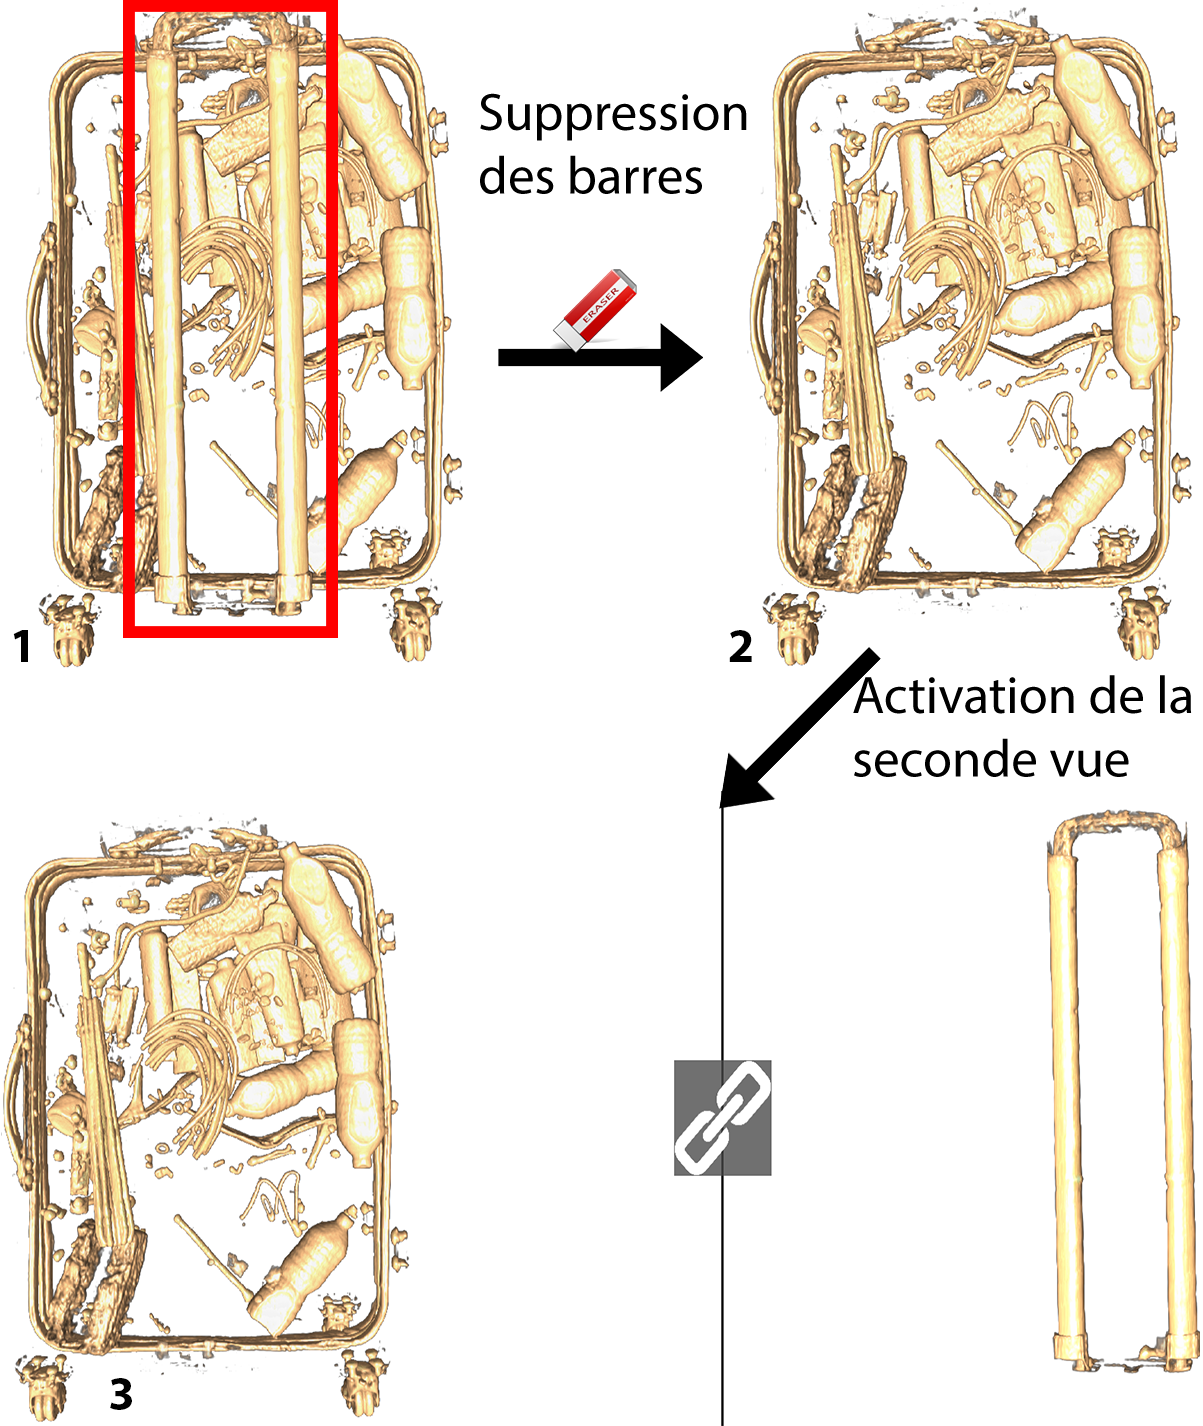
\includegraphics[width=0.9\textwidth]{Figures/deletionfr.png}
	\caption[ Résolution du problème d'occlusion en supprimant des objets d'une vue à une autre.]{Résolution du problème d'occlusion en supprimant des objets d'une vue à une autre. 1- L'utilisateur veut retirer les barres du bagage. 2- Après un double clic avec l'outil de suppression, l'objet est supprimé de la vue principale. 3- Après l'activation de la 2ème vue, les objets retirés sont visibles à l'extérieur des bagages.}
	\label{f:deletionfr}
\end{figure}

Deuxièmement, nous propageons la sélection dans toutes les directions. Pour chaque voxel rencontré, nous vérifions s'il est visible en fonction de la fonction de transfert en cours. Si le voxel est visible, nous continuons la propagation de la sélection. Nous nous sommes propagés dans les bagages en lançant de nombreux threads à partir de l'endroit où le premier voxel visible a été touché. Le nombre de threads dépend du nombre de processeurs logiques présents dans le matériel actuel. Chaque thread vérifie si ses voisins sont visibles et continue à se propager vers les voxels visibles. Cet algorithme de propagation s'arrête chaque fois qu'il n'y a plus de voxels visibles ou se propager, voir \autoref{f:deletionfr}.




Vu que nous avons développé ce système avec quatre agents de sureté, nous avons pu valider l’utilité de chaque technique développée. Grâce à un processus interactif, les utilisateurs ont donné leurs commentaires tout au long du processus de développement, ce qui a aidé à évaluer et à guider les techniques d'interaction proposées. Le feedback était principalement positif et les utilisateurs n'ont rencontré aucune difficulté particulière avec notre système. Les utilisateurs ont surtout apprécié l'interface simple avec peu de widgets et le nombre réduit d'interactions. Étonnamment, les utilisateurs étaient très intéressés à utiliser la fonction de transfert. L'histogramme et sa fonction de transfert ont également été appréciés même si la technique correspondante n'est pas simple à comprendre. Nous supposons que notre interface motive les utilisateurs à en apprendre davantage sur la technique derrière elle. Les utilisateurs ont également mentionné la nécessité d'afficher la densité réelle (la valeur numérique) de l'objet sélectionné. Ils demandent également à plusieurs reprises si la couleur affichée correspond à celle actuellement utilisée dans les paramètres opérationnels. Cela confirme le fait que les utilisateurs sont disposés à conserver certaines fonctionnalités existantes et préfèrent utiliser un système qu'ils connaissent déjà.
Les utilisateurs ont également apprécié nos exigences de conception avec des transitions en douceur et des investigations incrémentielles des bagages.
Toutes ces observations et évaluations qualitatives méritent d'être validées par des évaluations appropriées qui ne relèvent pas de cette étude.
Notre système est entièrement fonctionnel et interactif pour effectuer des explorations de bagages. De nombreuses améliorations peuvent encore être apportées afin d'améliorer ses utilisations en termes de nouvelles interactions et de réduction du temps d'exploration.
Techniquement parlant, la sélection du point de vue adéquat peut être améliorée avec plus de 6 faces étudiées. Mais dans la pratique, ce paradigme simple reste approprié. Si le point de vue calculé n'est pas entièrement satisfaisant, on peut faire pivoter manuellement les bagages. Néanmoins, l'algorithme développé ne fournira pas nécessairement la meilleure solution (l'occlusion la plus basse) mais une solution satisfaisante.
\par Notre objectif était de développer des interactions innovantes pour effectuer l'exploration des bagages mais nous n'avons pas vraiment pris en compte l'optimisation de la durée de l'exploration. La manipulation du volume 3D peut prendre du temps, tout comme nos nouvelles techniques d'interaction. Nous pensons que ces techniques ont un grand potentiel, car elles permettent d’explorer plus en détail un bagage suspect. Les techniques d'investigation existantes (avec l'image 2D aplatie) permettent de détecter rapidement et efficacement des bagages «propres». Nos outils peuvent alors être une bonne solution pour enquêter davantage sur une menace potentielle avec plus de temps disponible.


\NewPage

\section{ Preliminary user study }
During the first months of my thesis, I carried out a user study of eye tracking devices to build interactive systems for Air Traffic Controllers. \textbf{ The purpose of that was quite similar to the one I describe in this chapter: \textit{Provide fluid and fast interactions to ease the tasks of the users.} } The results of this work have been published in the proceedings of the HCI-Aero conference in 2016. As with baggage inspection, the operators deal with a critical task with a lot of cognitive workload. In addition, many lives can be affected by a single bad decision. Theses reasons were the main motivations to try to simplify and modernize these systems (Air traffic control interface and Baggage visualization software). 


While the mouse is the main input device for interacting with different screens, many alternatives do exist. In this work, we reported our exploratory study with the usage of
eyes as a new input device for Air Traffic Control systems. Our investigations, based on a user-centered design, included a study of the activity, a classification of interaction
techniques based on eye tracking systems, and finally a working prototype with the evaluations of the developed interaction techniques. Our goal was to investigate gaze usages
as a means of interaction, and give recommendations for future development of Air Traffic Control systems.


The activity of air traffic control is complex. Operators use many interactions techniques with dedicated IT systems to ensure the traffic flow with respect of security and
optimization concerns. Air traffic activities is constantly evolving. Air traffic
controllers, responsible for ensuring the safety and the fluidity of air traffic, have to deal with more and more information that could cause a significant increase in their
workload. However, whether in control tower, approach or even in En-Route control center, air traffic controllers have many tools in addition to the radar screen. Their
workspace is thus the scene of an accumulation of interaction devices (mainly mice and touchscreens).

\subsection{ Contextual observations }

In the following, we briefly describe the controller tasks within the three previously defined contexts. The activity of en-route and approach controllers [16] is mainly to maintain a safe distance between aircraft, and to guide them with traffic fluidity concerns. For this, the airspace is divided into sectors, each sector being the responsibility of one controller pair. When a flight goes through an area, controllers guide
the pilot by giving him or her orders (clearances) for heading, speed or altitude, until the flight reaches an adjacency sector where other controllers will be in charge of
this aircraft. In a typical environment, two controllers are seated in front of a control position, specially designed to support their job. A traditional position includes a set of
main subsystems: two radar screens (one for each controller), paper strips shared by both controllers (for systems using the strips) displayed on a horizontal table.

\subsection{ limiting factors }

With current systems, controllers are able to perform many
different types of interaction. This allows in particular to
obtain aircraft details, to setup the radar configuration or to
share information with other controllers. During the
observation sessions, we extracted some controllers frequent
interactions with existing systems:
\begin{itemize}
\item pan and zoom to set the radar view configuration,
\item entering a clearance,
\item distance computation between planes using the "alidade",
\item display of the separation distance between aircraft,
display of velocity speed vectors (position of the aircraft in
3, 6, or 9 minutes).
\end{itemize}

We have identified a number of limiting factors for these
interactions. Although navigation is available in the radar
image (pan and zoom), it still does not allow to see the
calling planes located outside of the displayed area. This
view configuration is done by clicking on the buttons located
in a context menu. Other features are accessible via a toolbar
or a shortcut menu. This is for example the case of the
alidade (measuring the distance between two aircraft), which
is performed by selecting it on the tool bar on the left of the
radar display (Figure 1) and then plotting on the map the line
representing the distance to assess the distance using a drag
with the left mouse button.
In conclusion, many interaction requires the mouse device with
numerous manipulations (reach the mouse, find the menu
location, select the appropriated item, perform selections and mouse drags, etc.)

\subsection{Interactions}
After the brainstorming, we built prototypes (\autoref{e:prototype}) that were
evaluated during a design walkthrough session with 3
confirmed air traffic controllers.

 \begin{figure}
 \centering
	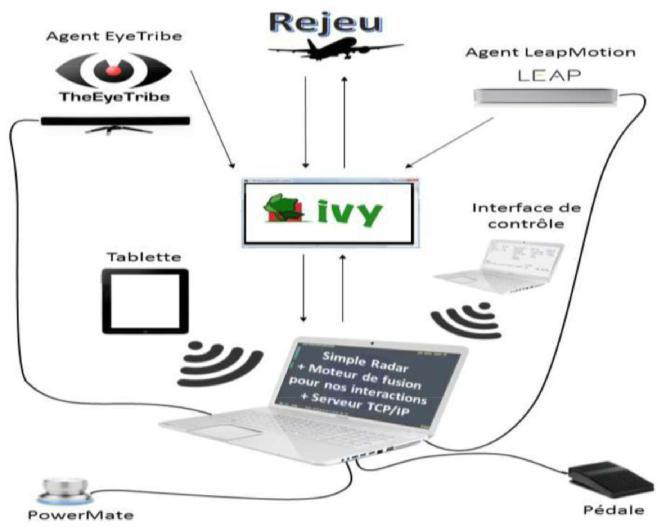
\includegraphics[width=0.95\textwidth]{Figures/prototype.png}
	\caption{ The architecture of the prototype}
	\label{e:prototype}
\end{figure}

\subsubsection{I1: Selection methods}
The selection of an aircraft is the first task an air traffic
controller shall achieve before interacting with it. To do this, different techniques of
interaction are possible and are shown in the following.

\begin{itemize}

\item \textbf{I1-1: The mouse (Existing Technic)}: We kept the functioning of this interaction which is already
implemented in existing systems, in order to compare the
eye tracker and the single mouse. (\autoref{e:})

\item \textbf{I1-2: The Dwell Time}: The Dwell Time is a technique that allows to change the state of a target (aircraft in this case) when looked for a certain period (\autoref{e:selectionState}).
\begin{figure}
 \centering
	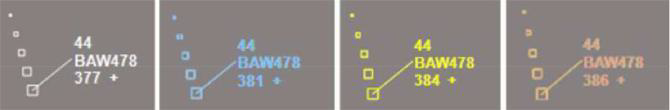
\includegraphics[width=0.95\textwidth]{Figures/selectionState.png}
	\caption{ The different states of an aircraft}
	\label{e:selectionState}
\end{figure}

Our prototype has two buttons, one for the validation and the
other one to cancel a previous validation. The appearance
and size of these buttons have been modified following the
remarks during the design walkthrough sessions. The
buttons are positioned in areas normally without traffic
(\autoref{e:selectionDwell}). The user must look at a plane: it will switch to
blue after a first timer (dwell time, 200ms). Then the user
simply look at the "validate" button for a certain period to
select the aircraft (it changes to yellow). To cancel the
selection of this aircraft, the user must again look at it, then it turns red, and if the user looks at the cancel
button for a certain period, the airplane is deselected (\autoref{e:selectionDwell}).

\begin{figure}
 \centering
	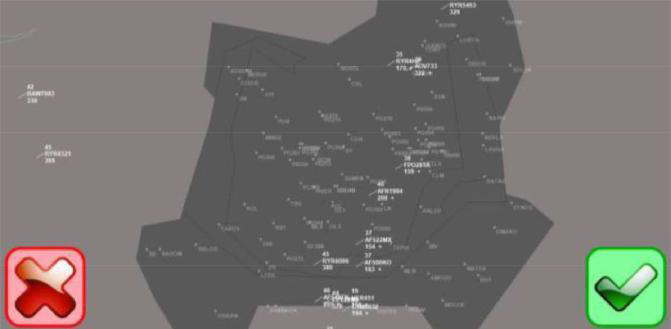
\includegraphics[width=0.90\textwidth]{Figures/selectionDwell.png}
	\caption{ Selection with dwell time}
	\label{e:selectionDwell}
\end{figure}

\item \textbf{I1-3: Buttons}: During the brainstorming session, it emerged that the best
option to select an aircraft is to use an external device
(button, keyboard or pedal, etc.). That is why we decided to
include this interaction in the final prototype.

\item \textbf{I1-4: Pedal}: This interaction is almost identical to the previous one, except that it offers the user a button that plays both the role of the "validate" and the "cancel".

\end{itemize}


\subsubsection{I2: Function Selection}
The methods of the function selection we implemented,
respond to the needs to obtain information on a plane, and
free the hands.
 
\begin{itemize}

\item \textbf{I2-1: Pulldown Menu}: This interaction is similar to the one existing in the current
systems. With a click on an aircraft, users have access to a
context menu offering several features. This interaction has
been developed for the purpose of comparison with the new
methods of selection that we propose (\autoref{e:selectionFunction}).
\begin{figure}
 \centering
	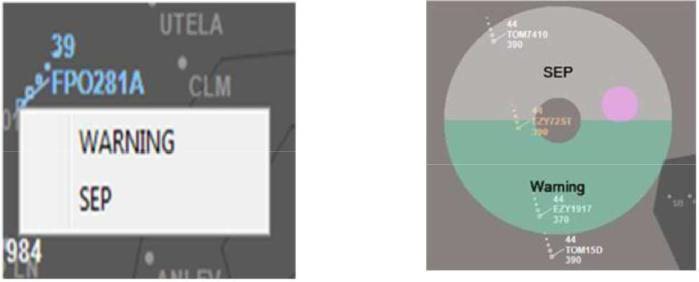
\includegraphics[width=\textwidth]{Figures/selectionFunction.png}
	\caption{
	A pulldown menu and a pie Menu.}
	\label{e:selectionFunction}
\end{figure}

\item \textbf{I2-2: Pie Menu and Dwell Time}: The advantage of the pie menu is that it appears at the exact
location where the user has selected the second aircraft.
Hence, the user can directly select one of the menu items.
However, following the remarks of some users, we have
increased the delay to 500ms before opening the pie menu.
Moreover, in order to respond to the need to keep all the
parts of the radar image visible, we opted for transparent
colors (\autoref{e:selectionFunction}).

\item  \textbf{I2-3: Pie Menu and Gaze Gestures}:In this interaction, the user must move his or her gaze from one of the menu items to the outside of the pie menu. This gaze gesture launches the warning function on the selected planes.

\end{itemize}
 
\subsubsection{I3: Zoom Methods}
These interactions respond to the need to freely navigate
through the radar image.

\begin{itemize}

\item  \textbf{I3-1: Pointer centered Scroll}: This interaction exists in some ATC interfaces (mainly interfaces without strip called "stripless"). The user acts on
the mouse wheel to zoom in or out. The zoom center is then
located at the mouse pointer. Also, it will help us to compare
the effectiveness of our new interactions.

\item \textbf{I3-2: Gaze centered Scroll}: As before, this zoom technique is based on the mouse, but
this zoom is not centered on the mouse pointer anymore, but
rather on the user's gaze location on the screen. In both
techniques, the zoom returns to its original level by clicking
with the mouse wheel.

\item \textbf{I3-3: Touchpad}: With the usual gestures made on a touch pad, the controllers can perform forward zooming (Pinch open) and backward
zooming (Pinch close) centered on his / her gaze.

\item \textbf{I3-4: Leap Motion}: The Leap Motion is a device that detects the movements and
aspects of the user's hands. We therefore used it to achieve
an interaction that is to approach or pull away the palm of
the hand to zoom in or out. When removing the hand form
the Leap motion's detection area , the zoom will return to
its original level.


\end{itemize}




\subsubsection{I4: Pan Methods}
Sometimes it is necessary for the controller to observe the
planes that are not necessarily displayed on the controller
screen. To do this, the user must perform lateral movements
(i.e. Pan) of the radar screen. These interactions respond to
the need to navigate through the radar image.

\begin{itemize}

\item \textbf{I4-1: The Mouse}: A first technique, which often exists in some air traffic control systems, is to make lateral movements with the mouse. The user clicks on the map then performs the
movements of "drag" to move it.

\item \textbf{I4-2: Touchpad}: This technique does not use the gaze but given the presence of the touchpad in the final prototype, we wanted to know if the users appreciated the fact to navigate through the map
with their fingers (as we can do it in Google Map
Application for Smartphone for example).

\item \textbf{I4-3: SmartPan}: Our goal was to use the eye tracker to observe directly a calling aircraft that would be out of the controller's screen.
For this, we have designed a system with voice recognition
to detect the corresponding call sign from calling aircraft. If
the calling plane is not within the area displayed on the
screen, the system automatically displays an arrow
indicating the direction toward this aircraft. The user then
has to look at the arrow (which gets yellow thanks to the eye
tracker), and a pan is automatically processed toward the
calling aircraft. This aircraft will be displayed in a different
color for easy identification (\autoref{e:smartPan}). Once the information
is taken by the controller, he or she just need to look in the
opposite direction of the arrow and the Pan
returns to its initial value. In user testing, we simulate a
calling plane with the control software.
\begin{figure}
 \centering
	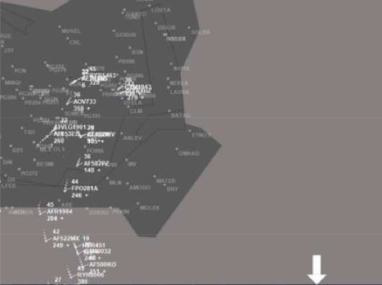
\includegraphics{Figures/smartPan.png}
	\caption{
	SmartPan: the arrow indicates a calling
aircraft outside the radar image.}
	\label{e:smartPan}
\end{figure}


\end{itemize}




\subsubsection{I5: Heat map}
The heat map is already widely used in other areas and
allows ATC to analyze the gaze of a user by recording the
history of the recorded gaze locations. These locations are
then transcribed in the form of a color gradient indicating
regions of interest on which the user focused on. When
controllers interact with each other to discuss a situation,
they often have to share information from the radar screen
and to highlight aircraft to clarify the situation. The idea
here is to use the heat map as a support to discussions and to
solve conflicting aircraft situations. When one of the
two controllers do not immediately identify the area his or
her colleague is talking about, one can press a button or a
key to display a heat map tracing the gaze history (about 20
seconds of past gazes) of the areas observed (\autoref{e:heatmap}). The
controllers can then have an overview of the specific
situation and find a solution to address it.

\begin{figure}
 \centering
	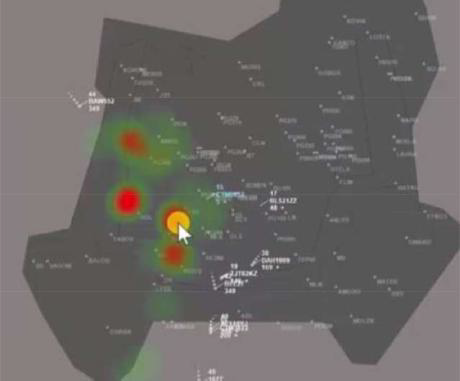
\includegraphics{Figures/heatmap.png}
	\caption{
	Heat map showing the most viewed areas +
improved magic pointer display the mouse cursor
inside the most viewed area}
	\label{e:heatmap}
\end{figure}

\subsubsection{I6: Improved Magic Pointing}
This interaction takes is root from the heat map
computation. Its goal is to display the mouse pointer at a
suitable location when the controller has to use it and thus
avoid too long mouse drag to reach the suitable pointing
target. To do so, just before the controller touch the mouse,
the algorithm computes the heat map. When the user moves
the mouse pointer, the system will display the mouse pointer
location at denser gaze location (\autoref{e:heatmap}).

\subsection{Evaluation of the prototype}
The first task was to change the state of two aircraft in a
conflict situation into "Warning". This task involved the use
of a selection method and the warning function. The second
task was to give a clearance (change of altitude or speed) to
an aircraft located in a dense traffic area. This task required
the use of a zoom technique. The third task was to give a
clearance to an aircraft located outside the area displayed on
the screen. We had the opportunity to test a method of pan.
And finally, the last task was to show the recorded gaze
location on the screen via a heat map.
Each of these tasks has been performed with each of the
proposed interactions including the techniques used in the
current ATC systems. At the end of each task, the user had
to give their opinions by filling a questionnaire asking a
qualitative evaluation of each of the interaction techniques.

The heat map was generally appreciated, especially by the
instructors. Indeed, they found that it would be very
interesting during the training courses of controllers in the
sense that this heat map would help them observe and
correct the visual path of apprentice. It is also a good help
for the other controllers who will be able to know if their
colleague is aware or not of a conflicting situation. The
zoom centered method on the gaze using the mouse wheel
was the method that received the most positive comments
from users.
Following user tests, many interactions have been improved
and new ones were created to best meet the needs of air
traffic controllers. To select an aircraft with only the eyes,
we designed another solution. When the plane is gazed, two
small labels appear on its side.

Regarding the selection of functions, the pie menu was not
easy to master, either with the selection of items via the
dwell time or worse through gaze gestures. In stressful
situations, involuntary actions could take place. To address
this, we proposed a validation of pie menu items via a button
or keyboard. We also added a visual feedback on the gazed
item in order to meet user' needs during the first test
session.
We developed new interaction techniques. The most appreciated
techniques were the gaze centered scroll, the SmartPan, the
selection combining the gaze and a switch, and the heat
map. The 2 main design recommendations emerging from
this study are, first, to validate the actions by a third device
for critical task; and second, to favor non penalizing
interactions in case of poor detection of the eye tracker. To compensate the loss of calibrations noticed during the
tests, we implemented an algorithm called Bubble Cursor  (see
\cite{Grossman:2005:BCE:1054972.1055012}). This algorithm consisting in computing the nearest
neighbor of the user gaze location. Thus, even if the eye is
not perfectly on one of the aircraft in the control area, the
nearest aircraft is still selected.



With almost the same motivations of providing fluidity and continuity between the interactions, we proposed a framework to support the interactive visualization of baggage.

\section{Introduction: Interactive exploration of 3D scanned baggage}
Volumetric data found in many fields, such as engineering, material sciences, medical imaging, astrophysics. Their exploration is not trivial, and heavily impacted by the users' needs. In most airports, security agents deal with such data exploration during baggage inspections. They use two types of fluoroscopic systems: X-ray and tomography scanning systems. X-ray system provides a flattened 2D baggage scan while tomography scanning system produces transversal scans, also called slices. 
Thanks to data processing (e.g. \cite{deans2007radon}), they can produce a full 3D scan (set of voxel with their corresponding density).
Our input data is a uniformly sampled multivariate field F : D $\longrightarrow$ V, D $\subset \mathbb{R}^{n}$ 
,V $\subset \mathbb{R}^{m}$ with n = 3 (volume) and m=1 (scalar field).



\section{Activity analysis}

During this thesis, I had the opportunity to intend to training courses for security agents' instructors, and to visit an airport (Toulouse-Blagnac Airport). These helped me to study the activity of security agents and get the users' needs. The training courses lasted 3 weeks. In fact, I studied weapons and Explosives, scan analysis methods, dissimulation techniques, and fluoroscopic systems functionalities. In addition, I spent 3 days among the security agents of Brink's at Toulouse-Blagnac Airport. In this section, first I describe the security agents' task by describing their equipment, the prohibited articles, and the protocol to analyze a scan. Next, I highlight their activity issues by showing the different error types, and the dissimulation techniques.

\subsection{Task description}

The airport security agents have many roles depending on their work position. They control people (the passengers, the flight crew, and the airport personnel), and the luggage at security checkpoints. The different work positions are:
\begin{itemize}
\item The reception, where the security agents check the documents and put the hand luggage on the treadmill of the X-ray machine,
\item viewing and detection of objects and luggage through X-rays,
\item pat-down search,
\item baggage inspection.
\end{itemize}
In this study, we focus on the threat detection through X-rays.

\subsubsection{The Equipment}

In most French airport, the security agents two types of fluoroscopic system: the tomograph, and the classic system. The classic fluoroscopic system provides a 2D scan of luggage on the one hand, and on the other, the tomograph can produce transversal scans in addition to the 2D scan. Some scanners are able to detect explosive automatically, they are called EDS (Explosive Detection System). The architecture of the classic system is composed of:
\begin{itemize}
\item a mechanical set comprising a frame, a conveyor, and a collimator,
\item a physical set comprising an x-ray generator, a detector, and detection cells,
\item the central unit,
\item and input/output devices (keyboard, screens).
\end{itemize}
When a luggage get in the frame, the x-rays are sent from the generator to the L-shaped detector through the luggage's components. The x-rays are attenuated depending on the molecular density of the encountered objects, which allows to receive different x-ray intensities on the L-shaped detector. Then, the different received intensities are processed to get the final 2D scan.
The final image does not keep the original colors, instead they use 3 colors (orange, green, and blue) to show the density of each encountered object. The orange color is used for low density matters which are mainly organic. In opposition, the blue color is used for high density matters which are mainly inorganic. The green color expresses the superposition of different kinds of materials or average density materials, see \autoref{f:image2d}.

\begin{figure}
\centering
	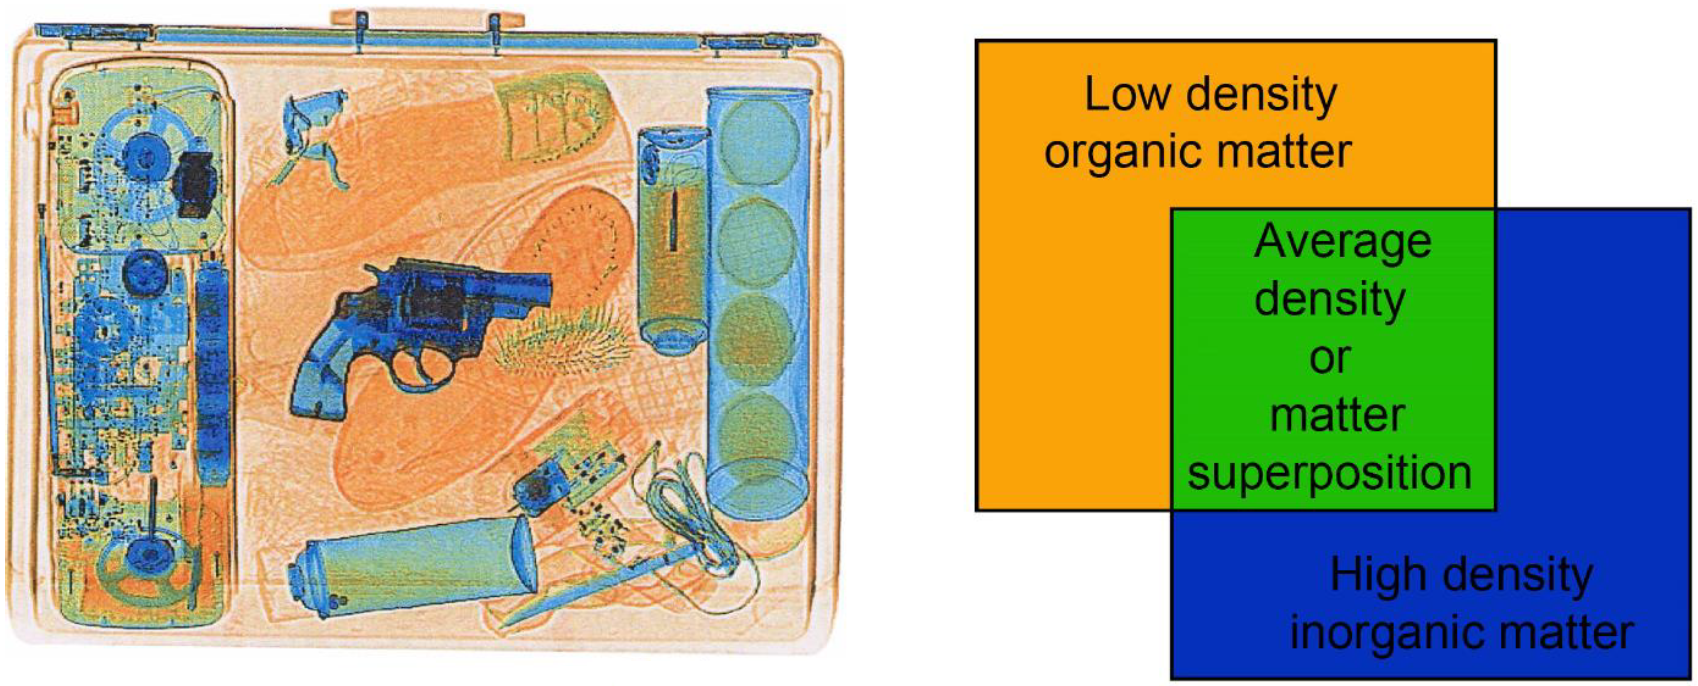
\includegraphics[height=5.2cm]{Figures/contour}
	\caption{ X-ray scan with the 3 standard colors (orange, green, and blue)}
	\label{f:image2d}
\end{figure}

\subsubsection{Prohibited articles}
Depending on the context, there are many prohibited articles. The aim is to avoid any kind of weapon to board in the aircraft. According to the regulations, weapons are items intended primarily to kill, injure, immobilize or reduce to impotence. The prohibited articles are:
\begin{itemize}
\item Guns, firearms, and any other equipment emitting projectiles,
\item Stun devices,
\item objects with a sharp tip or a cutting edge,
\item working tools,
\item blunt instruments,
\item explosive or incendiary substances and devices.
\end{itemize}
In addition to these prohibitions, some articles such as liquid, gels, and aerosols are restricted.

\subsubsection{Scan analysis}
Whatever fluoroscopic system is used, the security agents try to follow an analysis protocol to ensure any prohibited article is detected. This protocol is composed of 4 major steps, which are the global picture analysis, the in-depth analysis, the structure analysis, and the context.

\paragraph{Global picture analysis}


First, the security agent check whether the luggage is well placed. Indeed, the luggage should appear on the screen with \ang{45} of rotation. If it is not the case, a re-positioning is required. To avoid this issue, another agent must check the luggage positioning.
Next, the agent try to find out whether the luggage is complex or not. A luggage is complex when there is a superposition of usual objects and metallic materials. A complex luggage can hide threat and make them invisible. If possible, the complex luggage is opened and all troublesome objects are removed.

\paragraph{The in-depth analysis}


First, the security agent divides the luggage's component in groups. The aim is to reduce the risk of error. Indeed, smaller prohibited articles may be easily unseen. Then, the dark areas must be lightened up. To do it, the security agent can use functionalities such as high penetration or contour enhancement. If the area is still dark, the luggage must be opened to remove the serious doubts.
Next, the agent focus on the problematical shapes. A non-recognizable shape may be caused by a bad positioning. Any unrecognized object must be inspected by the agent. If any prohibited article is detected, the agent follows the procedure related to the threat. In addition, an organic matter superposed to an electronic device is considered as a sufficient reason to open the luggage. Liquids, gels, and aerosols should be less than 100ml otherwise they will be removed from the luggage. These liquids should be placed into a plastic bag.

\paragraph{The structure analysis}


During this step, the security agent compare each element of the luggage which must be symmetrical because of its industrial conception such us suitcase's wheels. If the symmetry is not respected, it is might be a clue to the deliberate luggage modification for dissimulating prohibited objects.

\paragraph{The context}


Depending on the context some articles are prohibited or not. The agent must be aware of his work position.
On an explosive detection system, the threats are already highlighted. The agent's job is to verify whether the threats are real or not.
In our study, we focus on a conventional system to provide new interaction techniques for analyzing 3D luggage scans.

\subsection{The activity issues}
There is many level of security in luggage inspection depending on the airport (between 1 and 6). Humans and machines work together to detect any potential threat inside the luggage. At the lowest levels of security, the security agents are in contact with the passengers, and therefore face 4 main operational constraints for safety and economical reasons: Facilitation, security, speed, and self-protection. 

First of all, The facilitation constraint implies that the security agent has to ensure a good user experience to the customers (the passengers). Second, they must prevent any potential threat to pass their inspection. In addition, they have to protect themselves from different kind of threats (ill-intentioned persons, parcel bomb). And finally, economical reasons oblige them to be fast enough in order to ensure a good flow. Therefore, the security agent face a trade-off between these four constraints, see  \autoref{f:constraints} .
\begin{figure}
\centering
	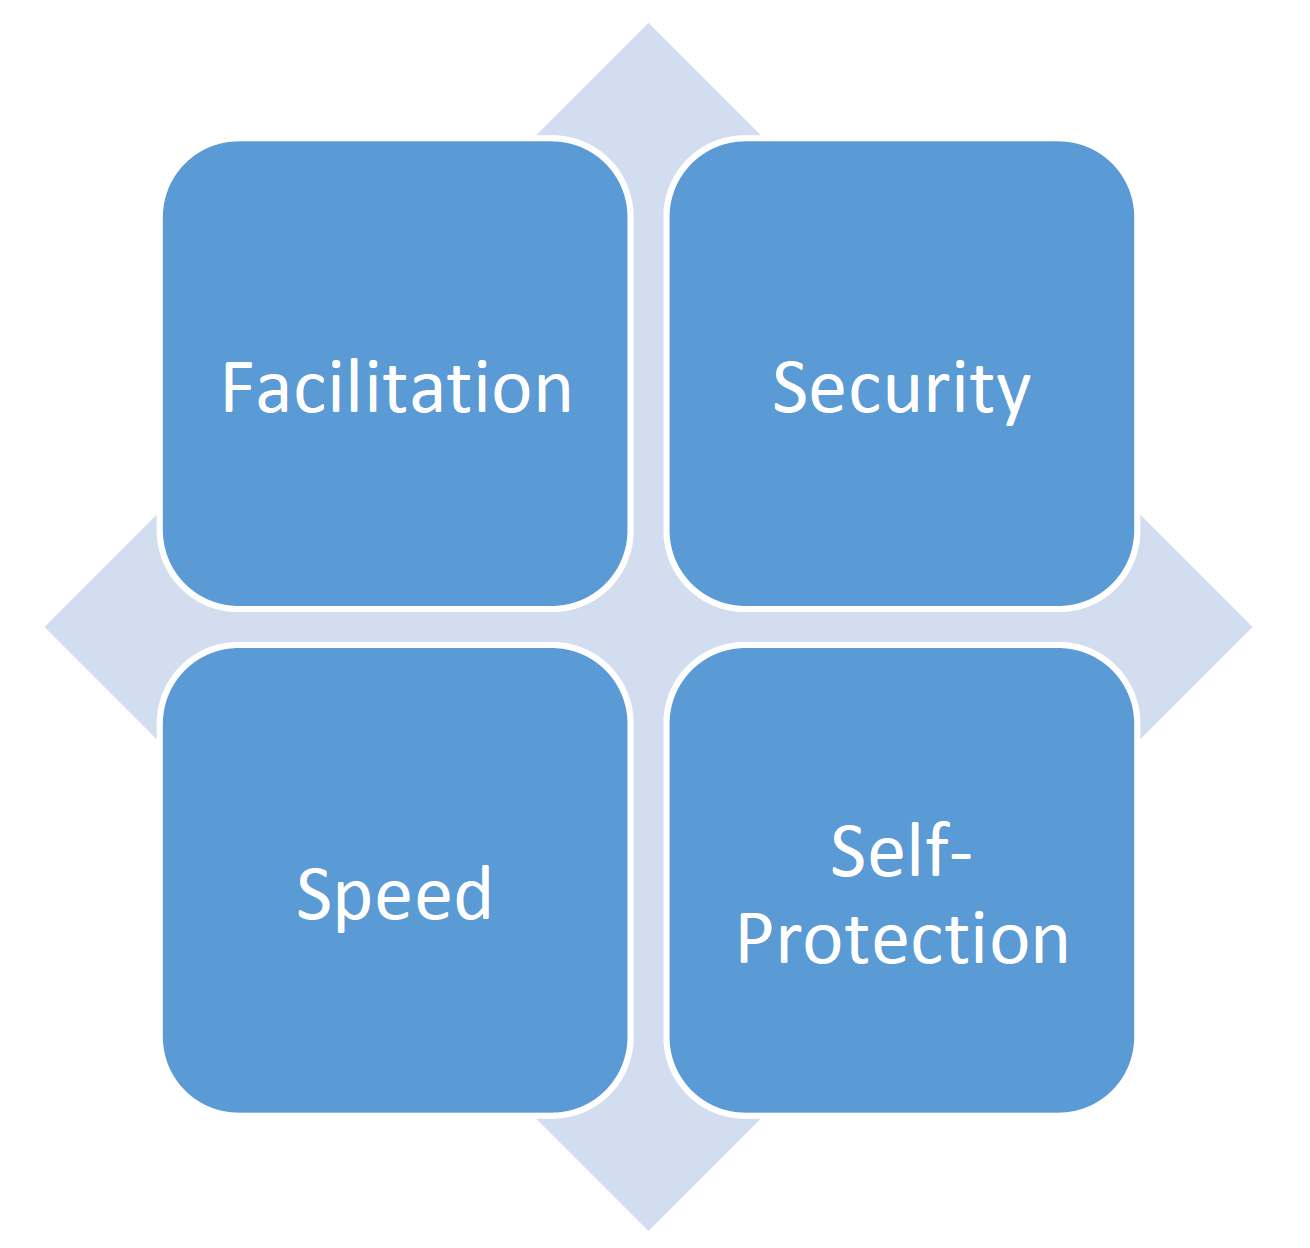
\includegraphics[height=5.2cm]{Figures/constraints}
	\caption{The operational constraints of the security agents.}
	\label{f:constraints}
\end{figure}



\subsubsection{ Error Types }


The security agents can usually do 3 types of error during the baggage inspection process.

\paragraph{Perception errors}

The security agent does not detect the right area to analyze. He is not focus on the troublesome area, see  \autoref{f:perception}.
\begin{figure}
\centering
	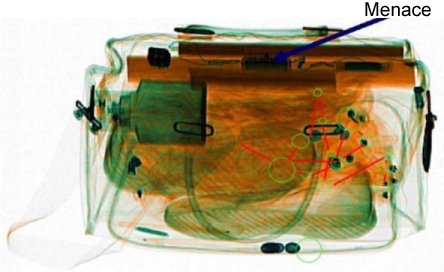
\includegraphics[height=8cm]{Figures/perceptionError}
	\caption{Perception error. The security agent do not notice the menace at the top of the image (the initiating system of an explosive) }
	\label{f:perception}
\end{figure}
\paragraph{Interpretation errors}

The security agent detects the right troublesome area but does not judge it as a potential threat. In other words, he is focused on the right area but cannot see the menace. The agents used to combine what they find out with their knowledge on real world objects stored in their memories. They have their own model of the situation, see  \autoref{f:interpretation}.
\begin{figure}
\centering
	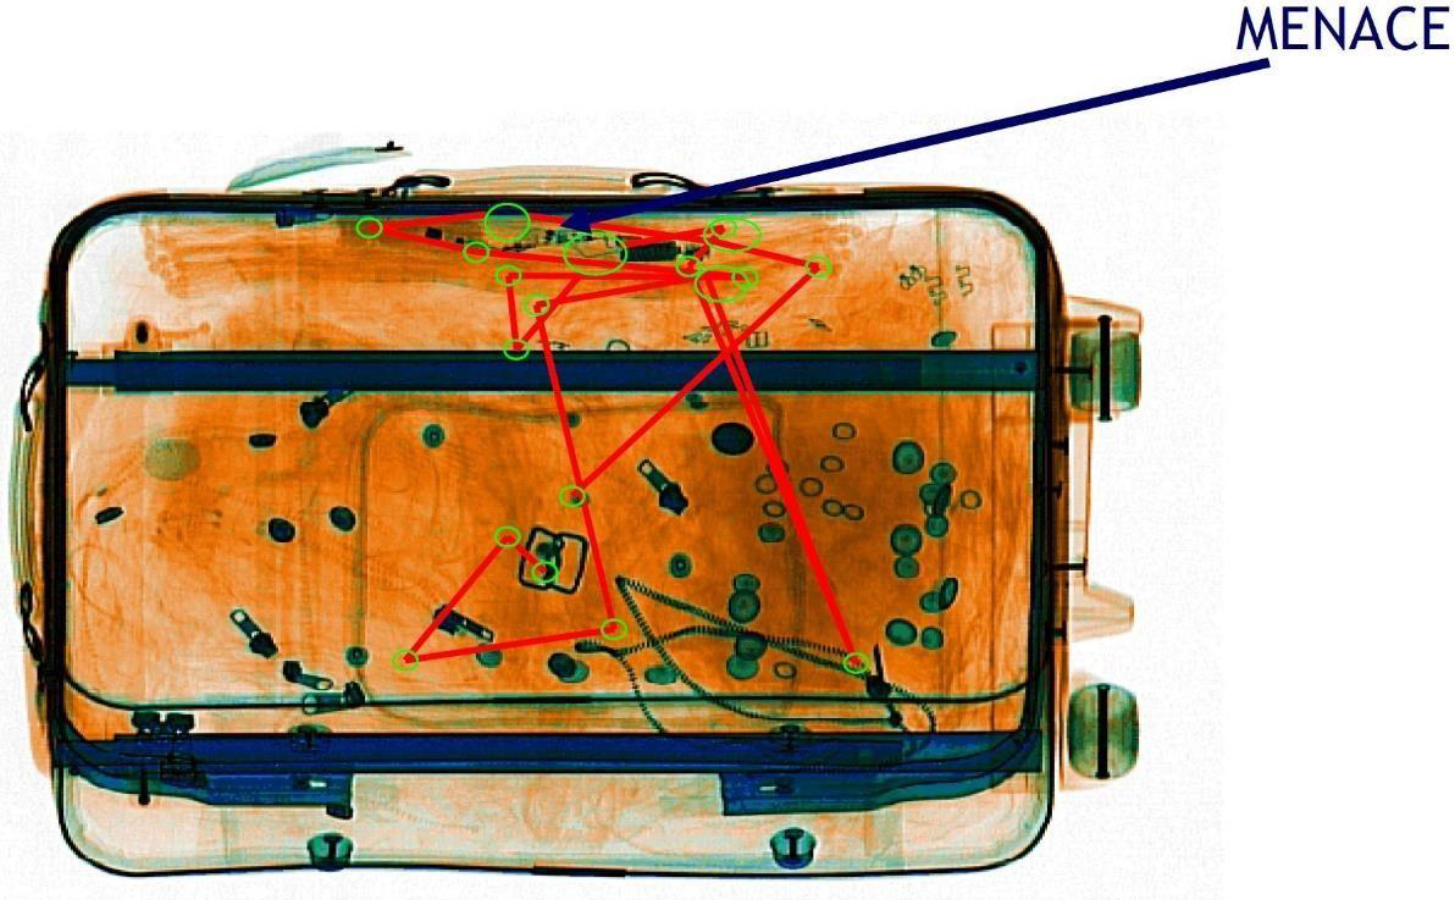
\includegraphics[height=8cm]{Figures/interpretationError}
	\caption{Interpretation errors. The security agent notice the menace at the top of the image do not interpret it as a threat (the initiating system of an explosive)}
	\label{f:interpretation}
\end{figure}

\paragraph{Decision making errors}
In this case, the security agent detects the right troublesome area with a good interpretation, but make a bad decision. It might be related to the context or the procedure knowledge.
In addition to these errors related to the agent, four hiding techniques can be used to bypass the security mechanisms. Those techniques are superposition, positioning, dissociation, and bait.

\subsubsection{ Dissimulation techniques }
Since the resulting X-ray scanned image only contains densities, it cannot display the material original colors. The standard color visual mapping uses 3 different colors (orange, green, and blue) to display the data density. Orange color corresponds to low density (mainly organic items). In opposition, blue color is used for high density items (e.g. metal). In the case of X-ray systems, green color corresponds to the superposition of different kinds of materials or average density materials (\autoref{f:image2d}). 

The displayed 2D scanned image can suffer from four issues.

\textbf{Superposition}: A threat (e.g. prohibited object like knife, cutter…) may be sheltered behind dense materials. Sometimes, it is possible to see through these blind shield using some functionalities such as high penetration (enhanced X-ray power) or image processing (contrast improvement),  see  \autoref{f:superposition}. 
\begin{figure}
\centering
	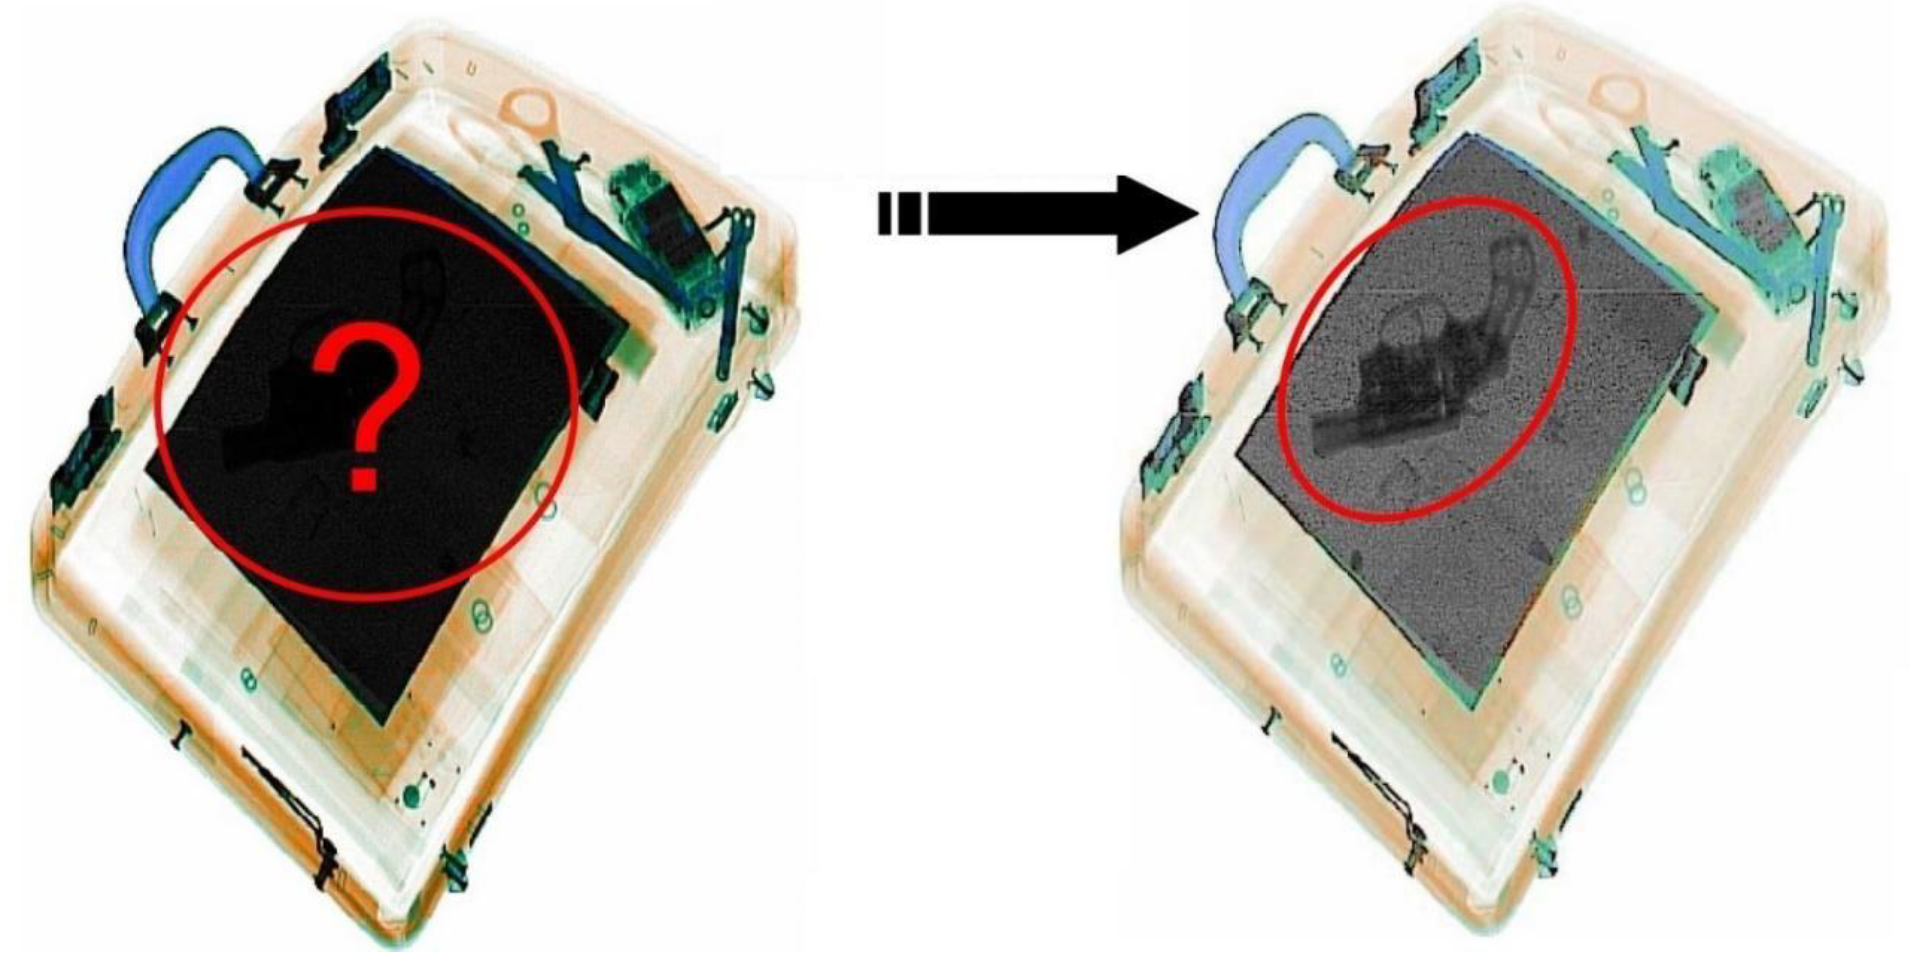
\includegraphics[width=0.95\textwidth]{Figures/superposition}
	\caption{Dissimulation by superposition}
	\label{f:superposition}
\end{figure}

\textbf{Location}: Depending on its location inside the luggage, a threat can be difficult to detect. Objects located in the corners, in the edges or inside the luggage's frame are very difficult to identify,  see  \autoref{f:location}.
\begin{figure}
\centering
	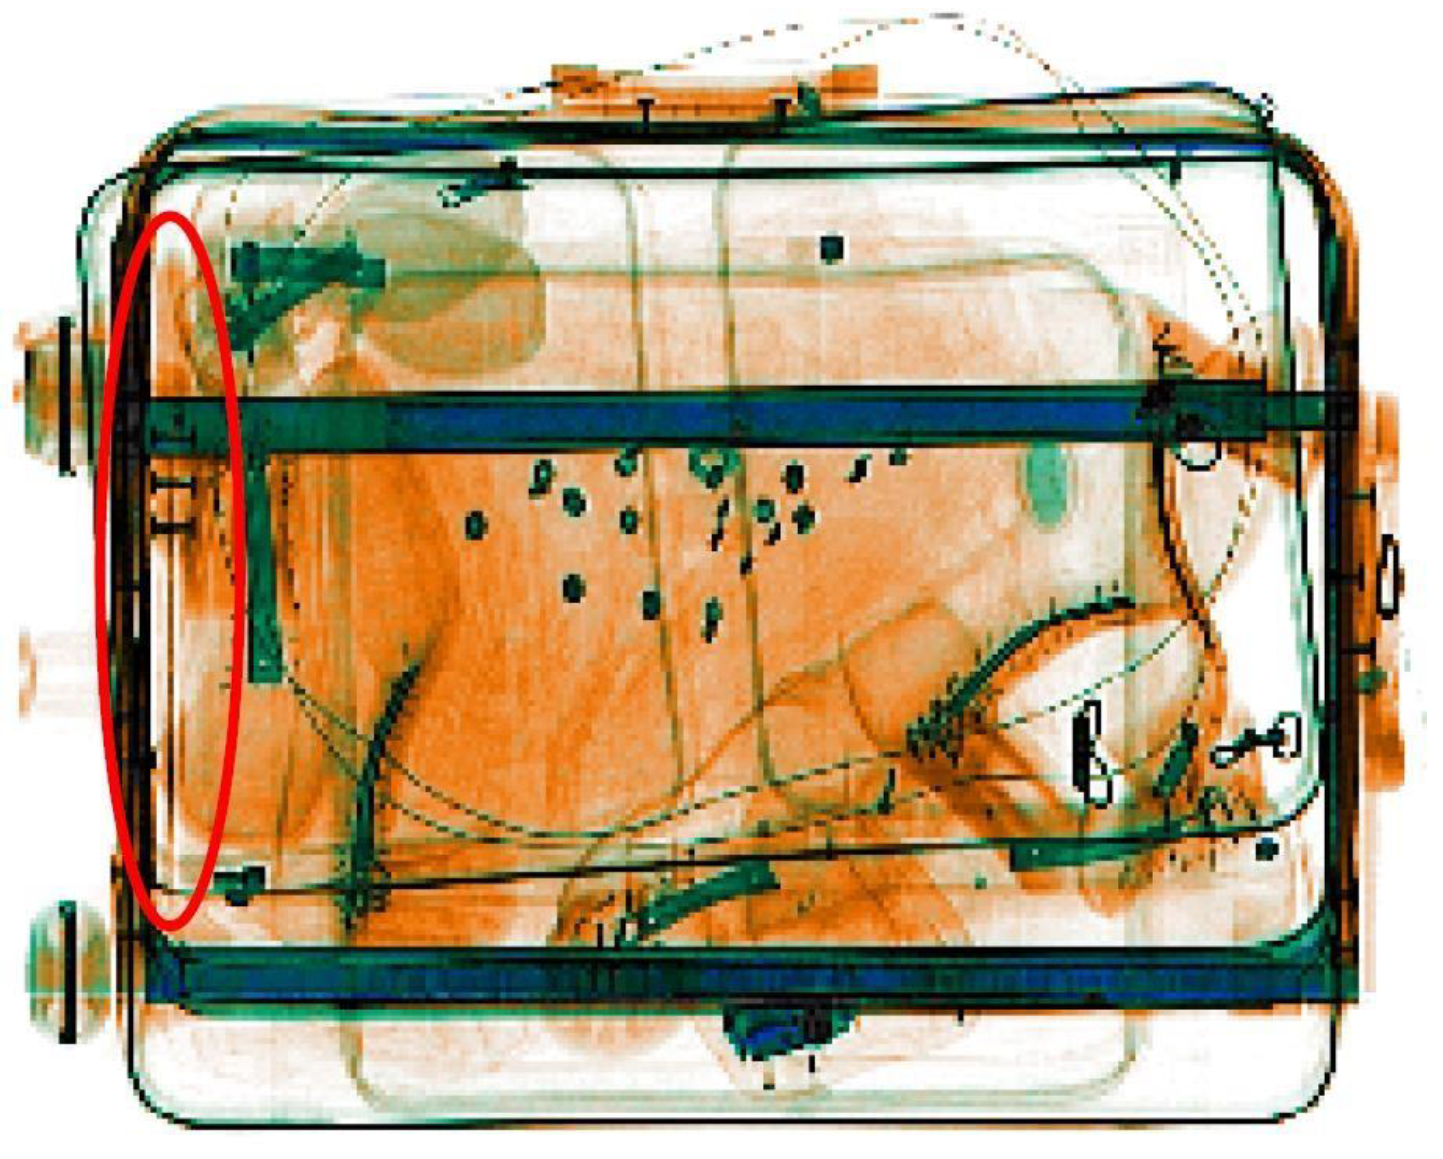
\includegraphics[width=0.9\textwidth]{Figures/positioning}
	\caption{Dissimulation by the location}
	\label{f:location}
\end{figure}

\textbf{Dissociation}: Another way to dissimulate a threat is to separate and to spread parts of it in the luggage (weapon or explosive are composed of many separated items like the trigger, the cannon...). This dissociation can be combined with other dissimulation techniques,  see  \autoref{f:dissociation}.
\begin{figure}
\centering
	\includegraphics[width=0.8\textwidth]{Figures/Dissociation}
	\caption{Dissimulation by dissociation}
	\label{f:dissociation}
\end{figure}

\textbf{Lure}: An ill-intentioned individual may use a lure to hide the real threat. For instance, a minor threat like a small scissors may be clearly visible and catch security agent's attention while a more important threat remains hidden, see  \autoref{f:bait}.
\begin{figure}
\centering
	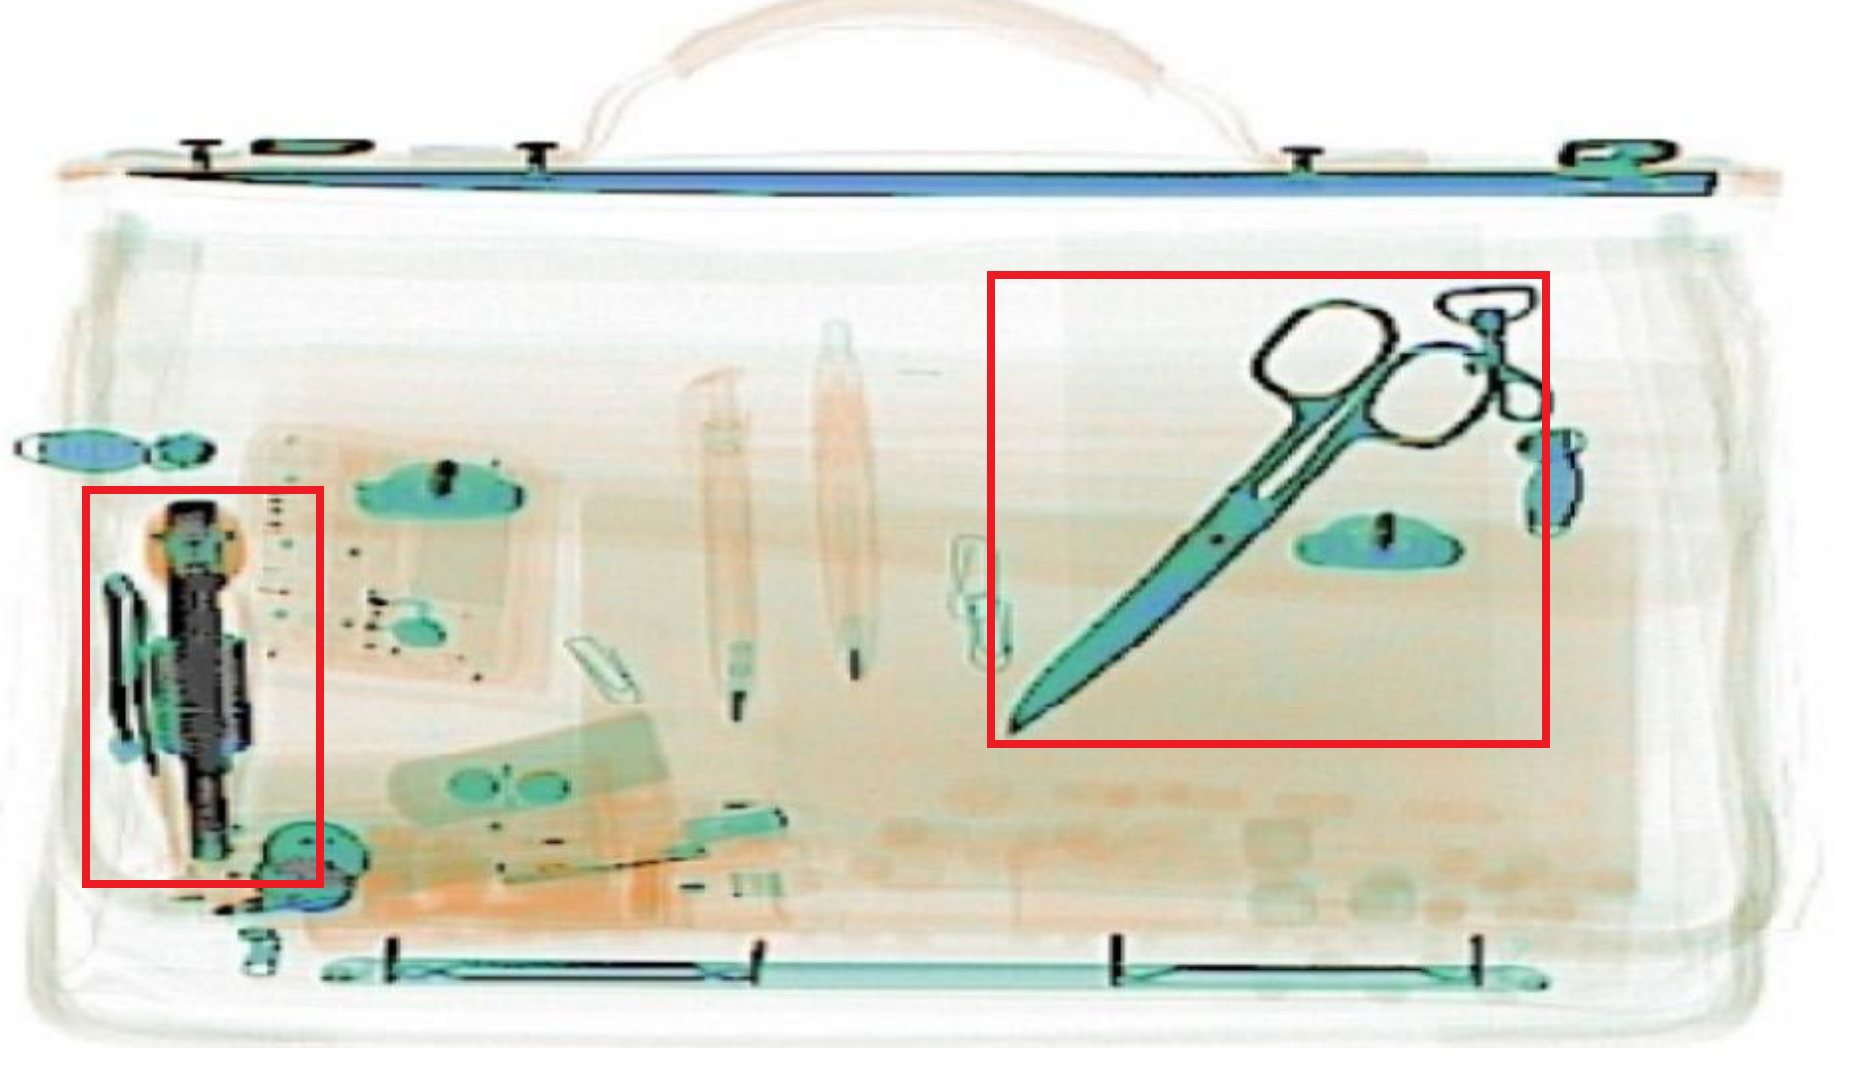
\includegraphics[height=8cm]{Figures/bait}
	\caption{Dissimulation using a bait}
	\label{f:bait}
\end{figure}

\subsection{ Requirements }


3D baggage scan exploration are one potential solution of such limitations, but to the best of our knowledge fiew previous existing system investigated this activity domain with interactive volumetric exploration tools (\cite{Li:2012:LVV:2425296.2425325}). Even if extensive works have been done in medical 3D scan exploration and manipulation ~\cite{preim2013visual}, there is a great opportunity to adapt and develop new interaction and data manipulation techniques to support 3D baggage exploration.

We performed on site observations with contextual inquiry (one day observation in one of the major French airport). We also conducted one brainstorming with four security practitioners from which we defined relevant use cases. Thanks to these analysis, we extracted a set of top level needs and requirements :

•	VIS: users need to visualize the content of the luggage.

•	EXP: users have to explore the baggage with interactive navigation system.

•	OCL: the system must provide tools to address occlusion issues; the
superposition of items inside the luggage hinders their visualization.

•	INT: User need to explore luggage with simple interactions. User knowledge is too limited regarding volumetric data processing to understand the involved techniques and their parameters.


Les tomographes génèrent des fichiers contenant toutes les densités rencontrées par les rayons X à travers les bagages. Ces fichiers contiennent généralement environ 30 millions de valeurs. Pour charger et afficher un tel ensemble de données dans un système interactif, nous avons utilisé la puissance de calcul parallèle de la carte graphique. Nous avons utilisé un programme écrit en C\# combiné avec la plateforme de calcul parallèle CUDA et un ensemble de techniques GPGPU. Pour afficher le jeu de données, nous avons utilisé un algorithme standard de diffusion de rayons. Les contributions de votre travail reposent sur de nouvelles interactions et leurs algorithmes associés.


\section{ Interactive exploration of 3D scanned baggage }

\subsection{Top Level Structure}

Our system is composed of one main view (Volume Visualization) and 5 sub views to control and customize it, see  \autoref{f:layout}. Our interactive system does not provide menu and every feature is directly accessible from this main view (\autoref{f:layout}).
The Volume Visualization can contain up to two views to ease interactions with the 3D scan. These views display the baggage and one can navigate through it (zoom, pan, rotation), manipulate its content (brushing, selection, deletion). These two views can be linked or disconnected in order to inspect selected objects with or without their context.
A smaller view called Overview shows the location of the investigated area. The overview is one-eighth the size of the main window and is located at its bottom right.
\begin{figure}
\centering
	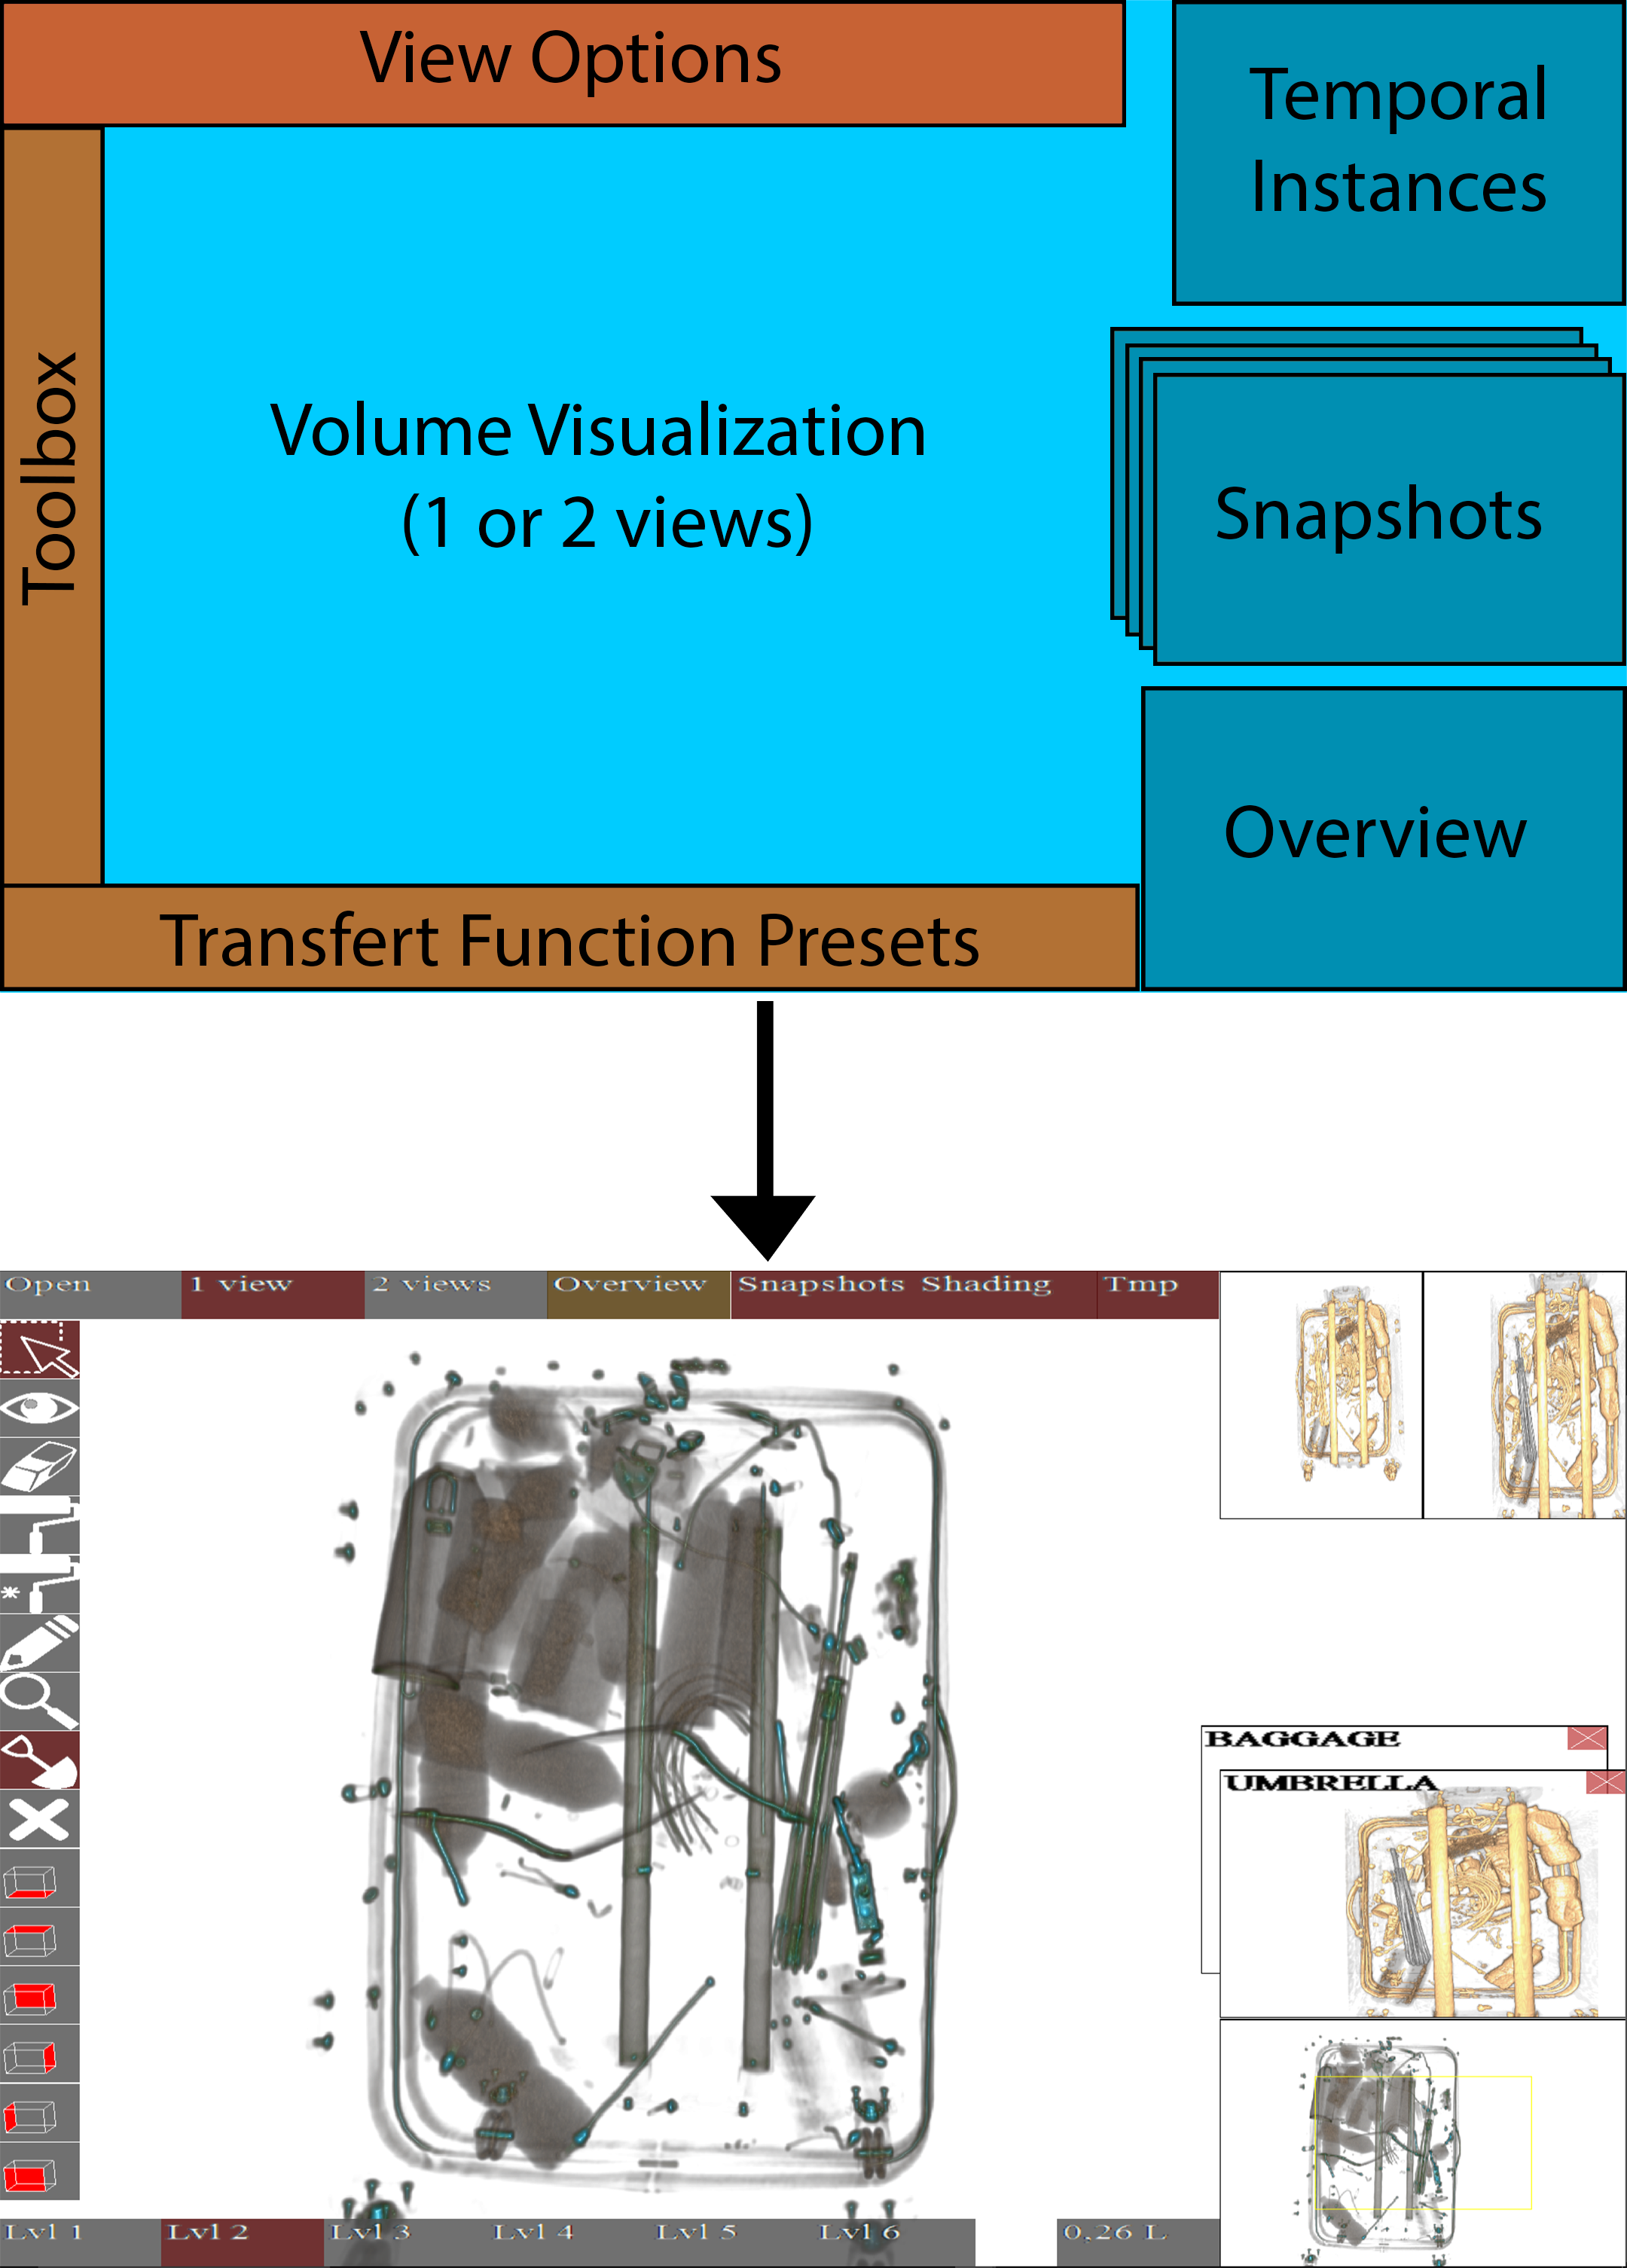
\includegraphics[height=14cm]{Figures/layout}
	\caption{Top level layout and screenshot of our Graphical User Interface. All the features are available through this GUI}
	\label{f:layout}
\end{figure}

Temporal Instances window, located in the top right of the interface, shows the current and the previous settings of the Volume Visualization. The current setting is modified when the user changes the transfer function or manipulates an object.
The Snapshot shows saved instances with their setting (pan, zoom, rotation, transfer function, selection, brushing).
The Toolbox contains every interactive tools to explore the baggage (brushing, selection, eraser, density picker, navigation tools).
Transfer Function presets contains six predefined settings ordered by their filtering power. Low level shows every density, high level only show high density values. 

This global layout can be customized thanks to View Options. One can display one or two views of the Volume Visualization, the Temporal Instances, the Snapshot and the Overview.

\subsection{Interaction techniques}

We used a multi touchscreen Wacom 24HD equipped with a stylus. Most of the developed interactions can be performed with every available modality: mouse, hand or pen.
\subsubsection{ Transfer function edition}	
Datasets such as two dimensional raster images or three dimensional voxel based representations are often processed for representation using a transfer function (TF) defined by a curve. 

Since airport security agents have a reduced time frame and limited knowledge of technical constraints, we defined six TF presets (\autoref{f:preset}). These presets only modify the TF transparency curve while keeping the same color mapping. These presets are ordered by their density filtering power: the first preset displays every density and the last one only highest density of the volume (i.e. metal). 

\begin{figure}
   \centering   
	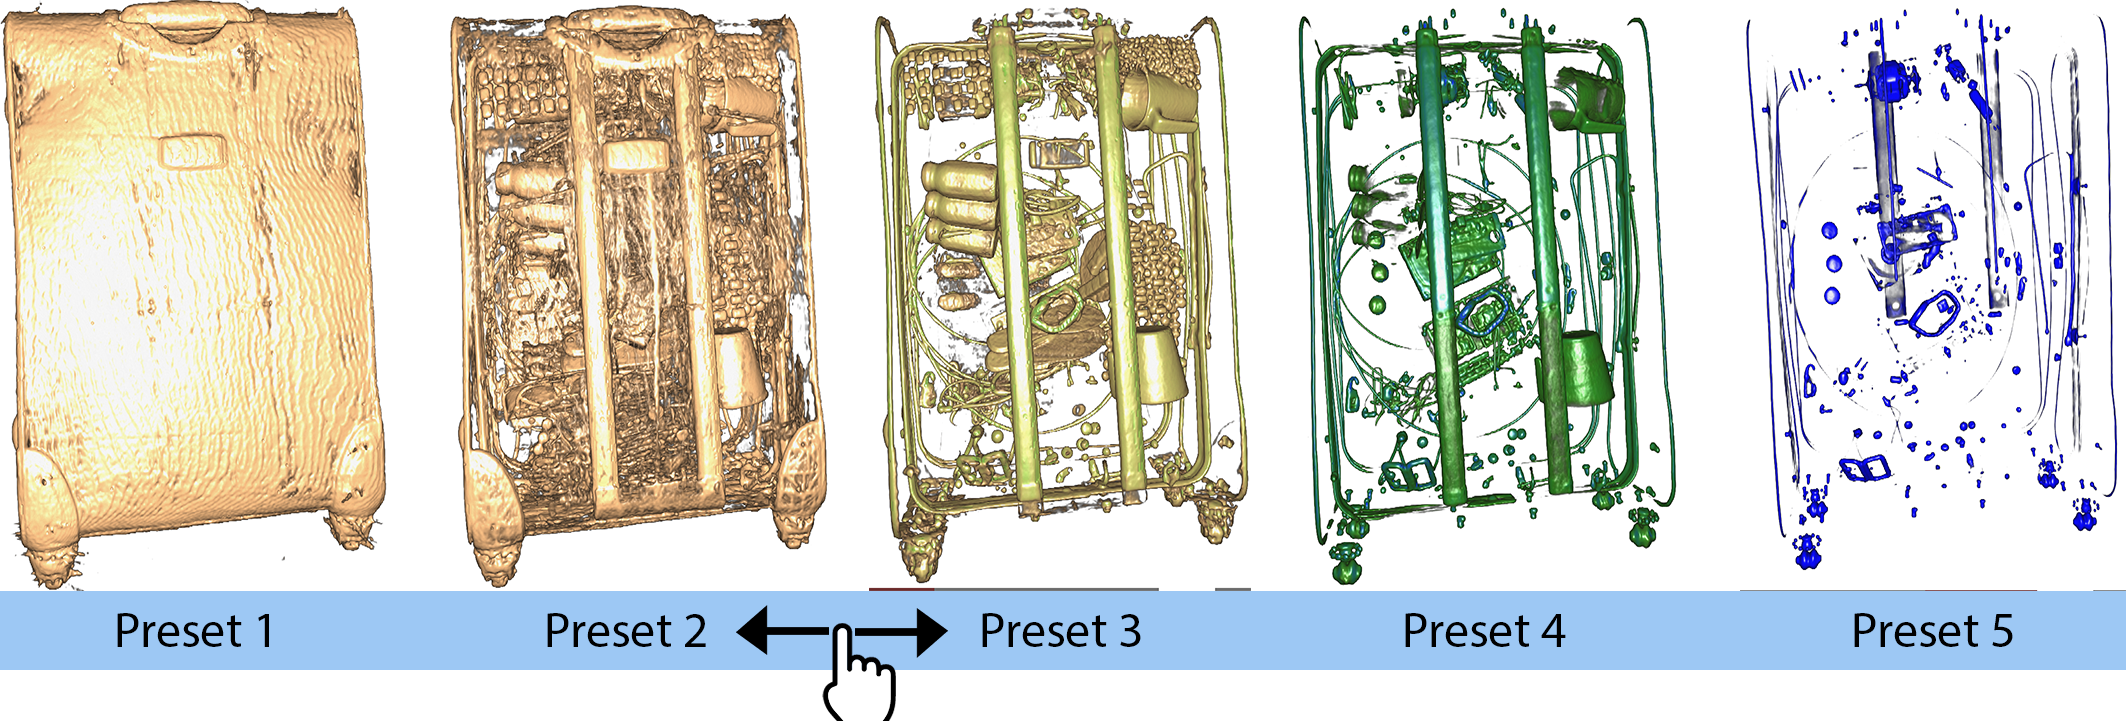
\includegraphics[width=15cm]{Figures/preset.png}
	\caption{ Transfer function presets and their continuous interaction. The high density materials are revealed by dragging from left to right on the presets }
	\label{f:preset}
\end{figure}
When clicking on a preset, the TF changes with a short transition (1 second) toward a new one. 
Finally, the user can select a transfer function located between two presets. To do so, the user drags from any location within the TF presets area until the volume visualization shows interesting features 

\subsubsection{ Objects selection and investigation}
In order to investigate in detail a specific object, one can isolate it, remove surrounding items to address occlusion issues, or find a suitable point of view (\autoref{f:menace}). This section details these interaction techniques which encompass the selection of  many objects.


\paragraph{	Selection of an object}
We developed three different ways to select objects with the three different modalities: hand, mouse or pen. When using his or her hand, the user has to double tap the desired object with his or her finger. When using the pen, the user must press the biggest button on the stylus while pointing at the target. Otherwise, the user has to double click on the target with the mouse pointer. After the target is selected, our system tries to find a better point of view to display the selected object with the minimum of occluded parts. The details of this algorithm will be explained in the technical part of this study. We use a smooth transition to rotate and zoom the baggage. 


\begin{figure}
\centering   
	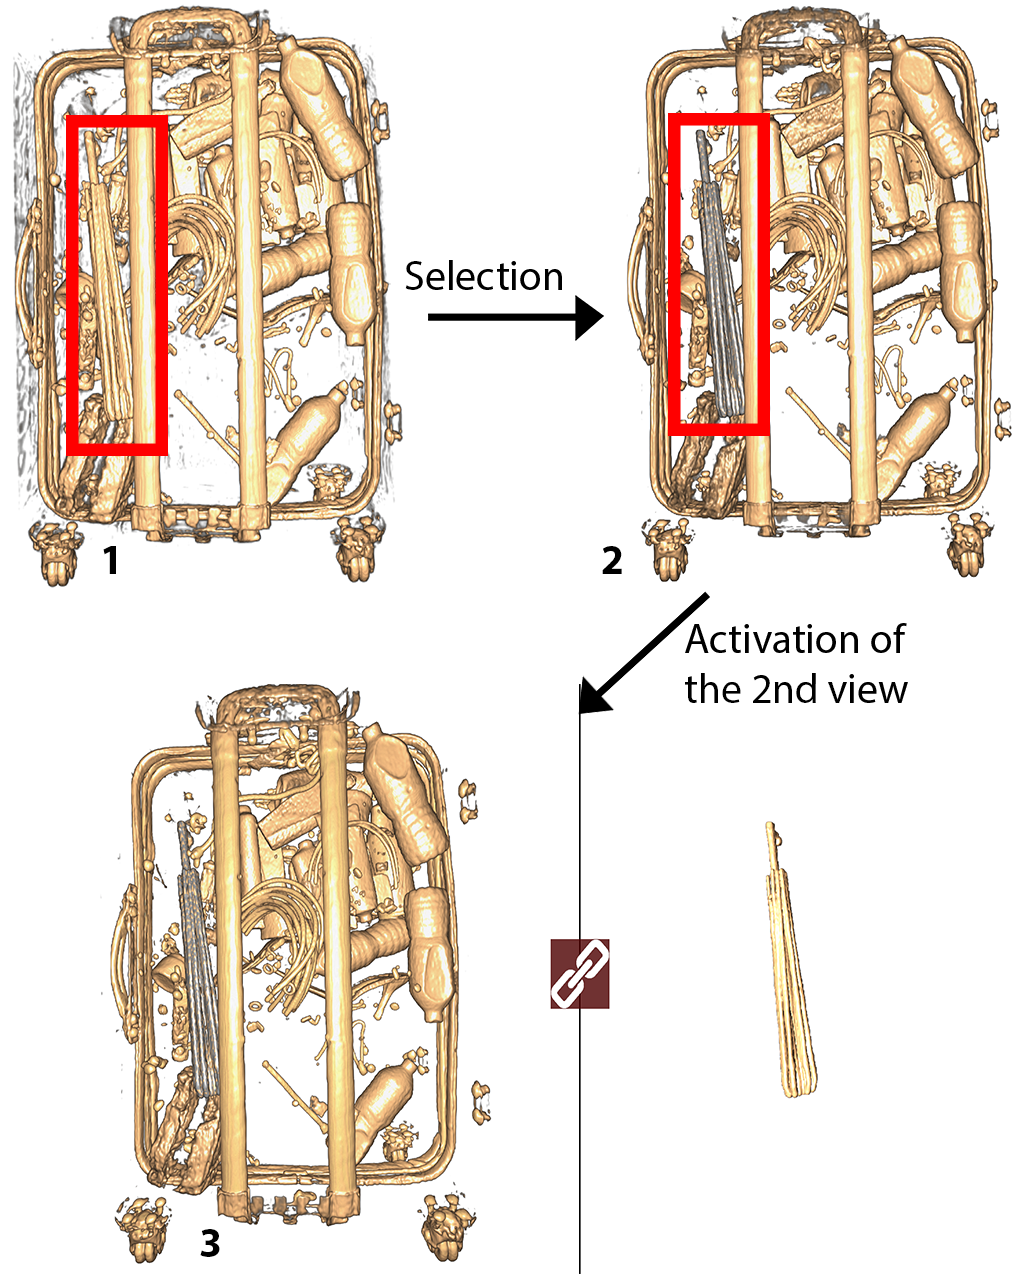
\includegraphics[width=9cm]{Figures/selection.png}
	\caption[Selection of an umbrella for further inspection.]{ Selection of an umbrella for further inspection.  1- The user wants to check an object looking like an umbrella. 2- After a double click, the object is selected and becomes gray as a feedback. 3- After the activation of the 2nd view, the user can manipulate the umbrella with or without the whole baggage. All the Selected items are also available on this second view. }
	\label{f:selection}
\end{figure}



If the user has activated the 2 views Volume Visualization (Button 2 views in the View Option panel), the selected object is isolated in the second view (on the right side of the main view \autoref{f:selection} ). The selection is incremental and many object can be selected one after another. To undo the selection, the user has to select the desired object in the second view.

\paragraph{Occlusion management}

In order to address occlusion issues, the eraser tool can interactively remove selected objects from one view to the other one. This interaction is similar to the selection interaction with all the modalities (mouse, hand, and pen). When using his or her hand, the user has to double tap the desired object with his or her finger. When using the pen, the user must press the biggest button on the stylus while pointing at the target. The user can also double click on the target with the mouse pointer. To restore a deleted object from one view, the user has to erase it from the other view, see \cite{hurter2017boolean}. This simple principle guarantees that every item of the baggage is always visible while addressing occlusion issues (\autoref{f:deletion}).

\begin{figure}
\centering   	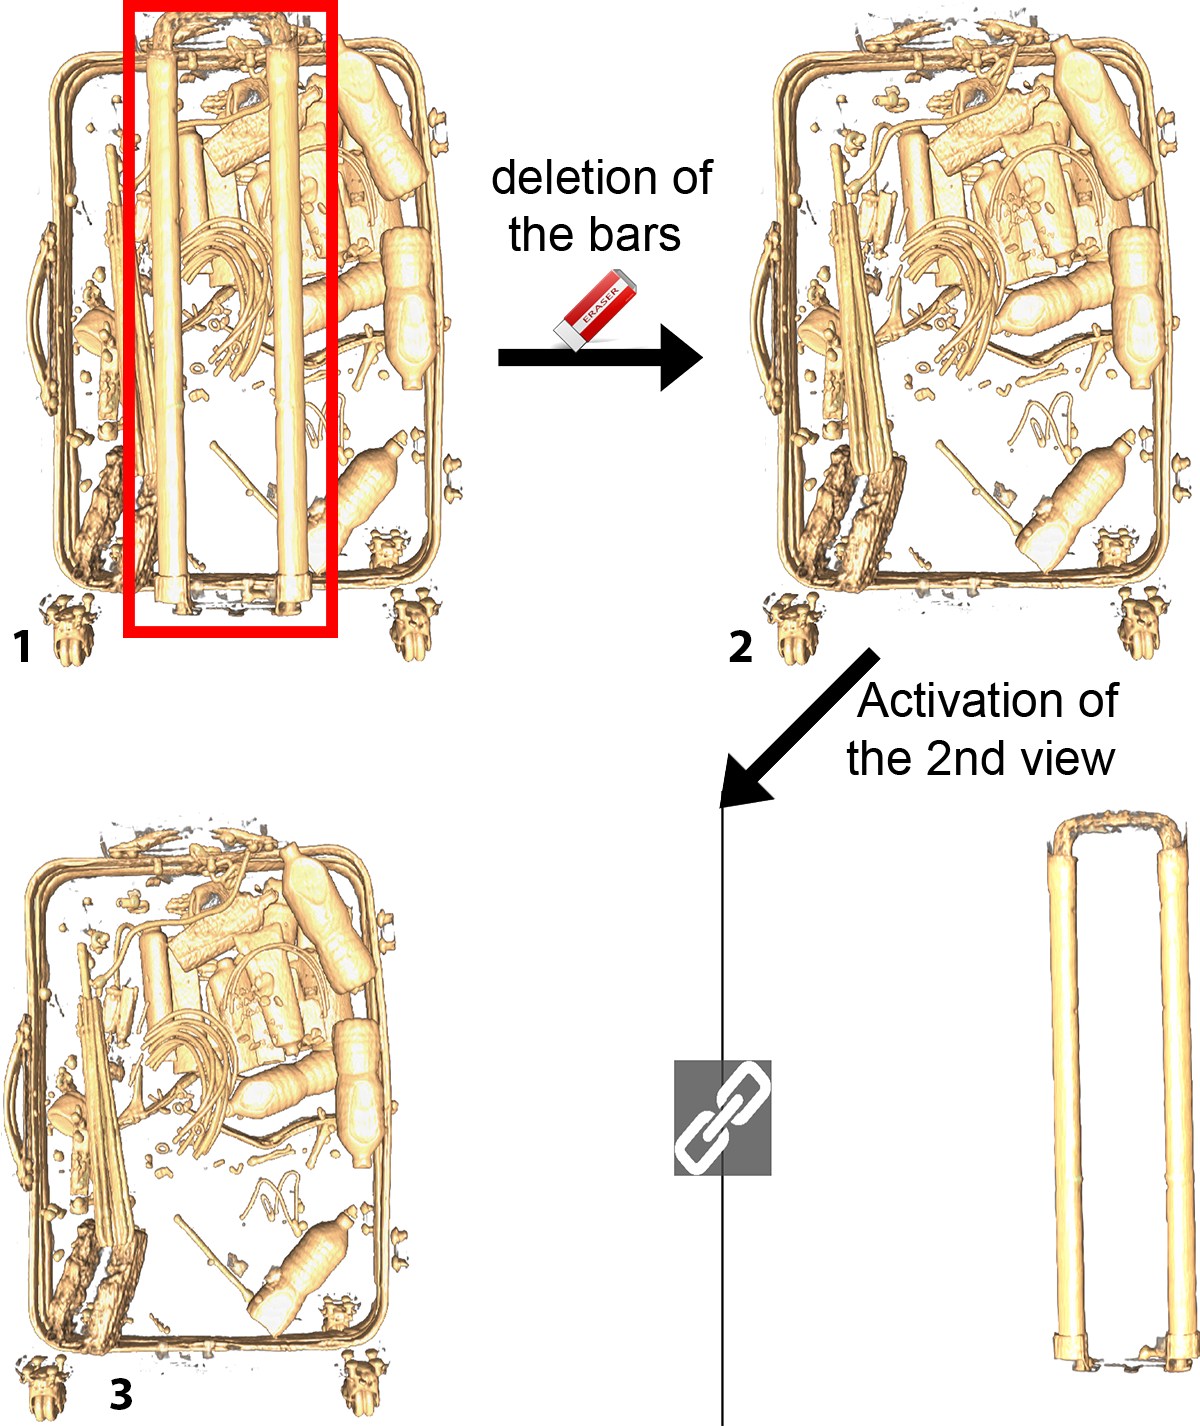
\includegraphics[width=9cm]{Figures/deletion.png}
	\caption[ Addressing occlusion issue by removing objects from one view to another one.]{ Addressing occlusion issue by removing objects from one view to another one. 1- The user wants to remove the bars of the baggage. 2- After a double click with the deletion tool, the object is removed from the main view. 3- After the activation of the 2nd view, the removed objects are visible outside the baggage.}
	\label{f:deletion}
\end{figure}

\subsubsection{Extended Brushing techniques}

\begin{figure}
\centering   	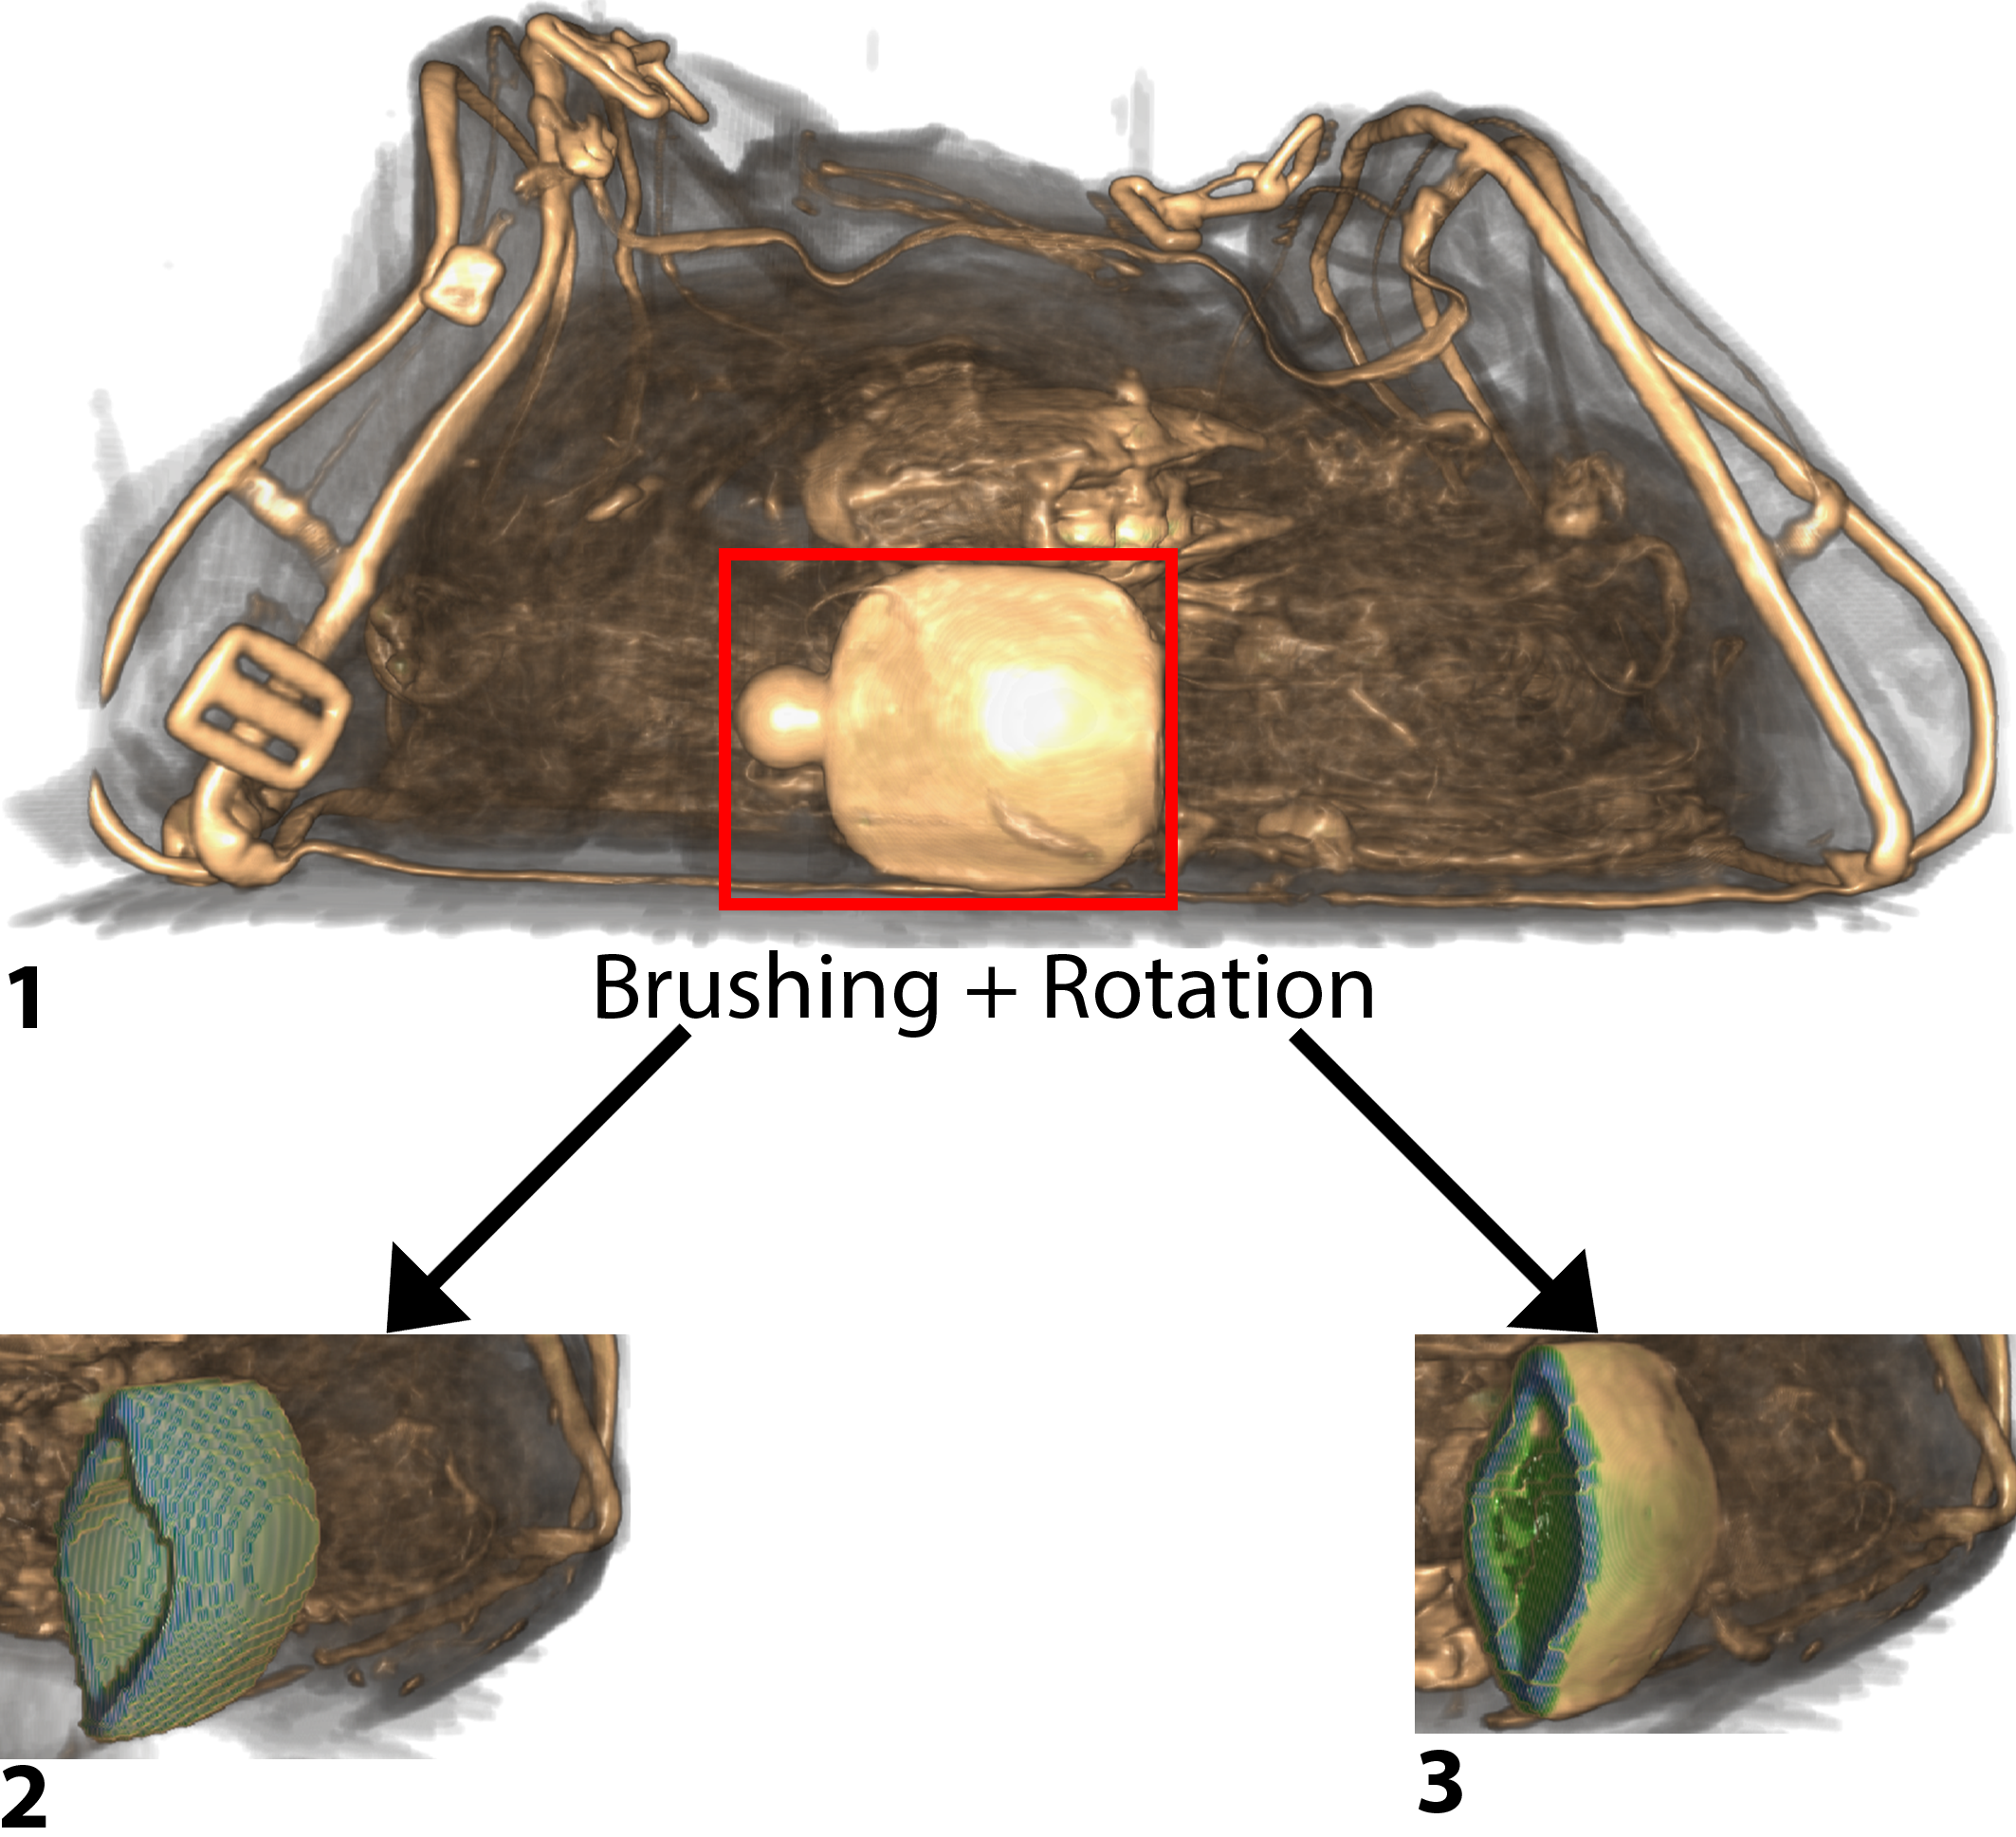
\includegraphics[width=9cm]{Figures/brushing-new.png}
	\caption[Brushing a bottle to see its content.]{ Brushing a bottle to see its content.  1- The initial baggage before brushing. 2- The result after using the old brushing technique: the content of the bottle has been removed too. 3- The result after using the new brushing technique: the content of the bottle is still visible. This brushing technique removes until it encounters an object out of the selected density range. }
	\label{f:brushing_new}
\end{figure}

Baggage is composed of low density items (e.g. fabrics, clothes, papers, organic objects…) and high density ones (e.g. metal, electronic components…). Low density items are more numerous and surround high density ones. In order to perceive a metallic object, one needs to remove or hide its surrounding low density items thanks to an adequate TF. Since TF is applicable to the whole volume visualization, the visualization of a metallic bottle will prevent to visualize its content (i.e. organic density). One cannot find out whether the metallic bottle is empty or not (\autoref{f:brushing_new}). To solve this problem, we developed two brushing techniques to explore the baggage by the mean of local removal of specific densities without modifying the TF.

\paragraph{Range Based brushing technique}

This interaction removes all voxels which are bounded in a user defined range. A range-slider is available on top of the transfer function (\autoref{f:brushing_range}). The user enables the brush tool in the toolbox by clicking on it and then the right button of the mouse removes the voxels beneath the mouse pointer.
Original brushing technique removes every voxel which is bounded in a density range and which is beneath the mouse pointer. In case of the exploration of a metallic bottle full of liquid, original brushing technique will remove the surrounding of the bottle as well as its content. To address this issue we developed a new brushing technique as if one digs into a baggage. This digging process will stop when a dense layer is encountered. This dense layer (e.g. the outer layer of a metallic bottle) will act as a shield to protect voxels located behind it (\autoref{f:brushing_new}).

 \begin{figure}
\centering	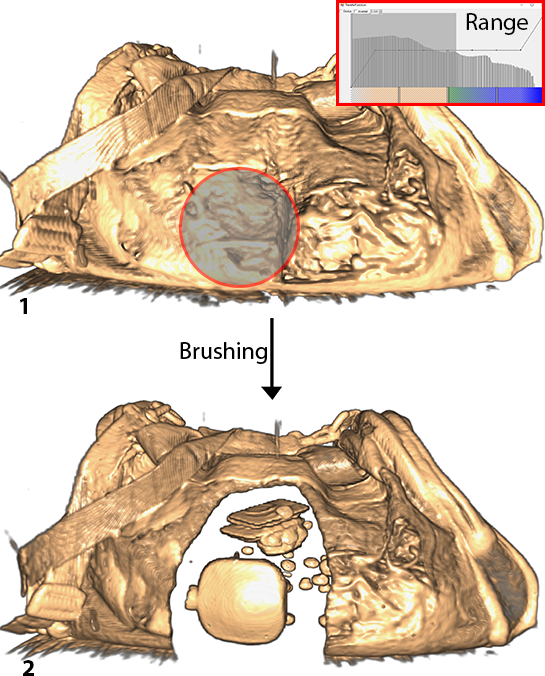
\includegraphics[width=9cm]{Figures/brushing-range.png}
	\caption[Brushing low density materials to see a metallic object hidden inside the baggage.]{ Brushing low density materials to see a metallic object hidden inside the baggage. 1- The baggage before brushing. 2- After a density range is defined, the users brushes a part of the baggage. This interaction reveals a metallic bottle.   }
	\label{f:brushing_range}
\end{figure}

\paragraph{Magic brushing technique}
This brushing technique has almost the same behavior as the range based brushing one. The main difference consist in the automatic range definition. This magic brushing removes all voxels with a lower density than the first one encountered at the beginning of the brushing process. This technique helps the user to directly define the densities he or she wants to brush. This technique avoid multiple interactions with the histogram and its range slider to define the range of brushable densities.

\paragraph{The cancellation of the brushing}
Our system offers the possibility to restore previously brushed areas. To do so, the user must select the brushing tool in the toolbox and hold the shift key while brushing over a given area. The restored densities are those defined by the histogram range slider. This restoring processing does not act as the range brushing technique and the sheltering effect (dense layer provides to brush behind it). Every voxels within the range are restored in order not to confuse the user.

\subsubsection{Snapshots}
Our system can store visual configurations thanks to snapshots. These snapshots are displayed on the right of the main view and record the current rotation, the zoom, the pan and the current transfer function.
To take a snapshot, the user must press the space bar. A name can be given to any snapshot using the keyboard. This name is displayed on the top left of its thumbnail. The user can restore a saved object by clicking on its snapshot. When a snapshot is selected, the system animates the view from its current state to the selected snapshot (pan, zoom and transfer function linear interpolation). A snapshot can be deleted by clicking on the close icon located on its top right (\autoref{f:snapshots}).
 \begin{figure}
 \centering
	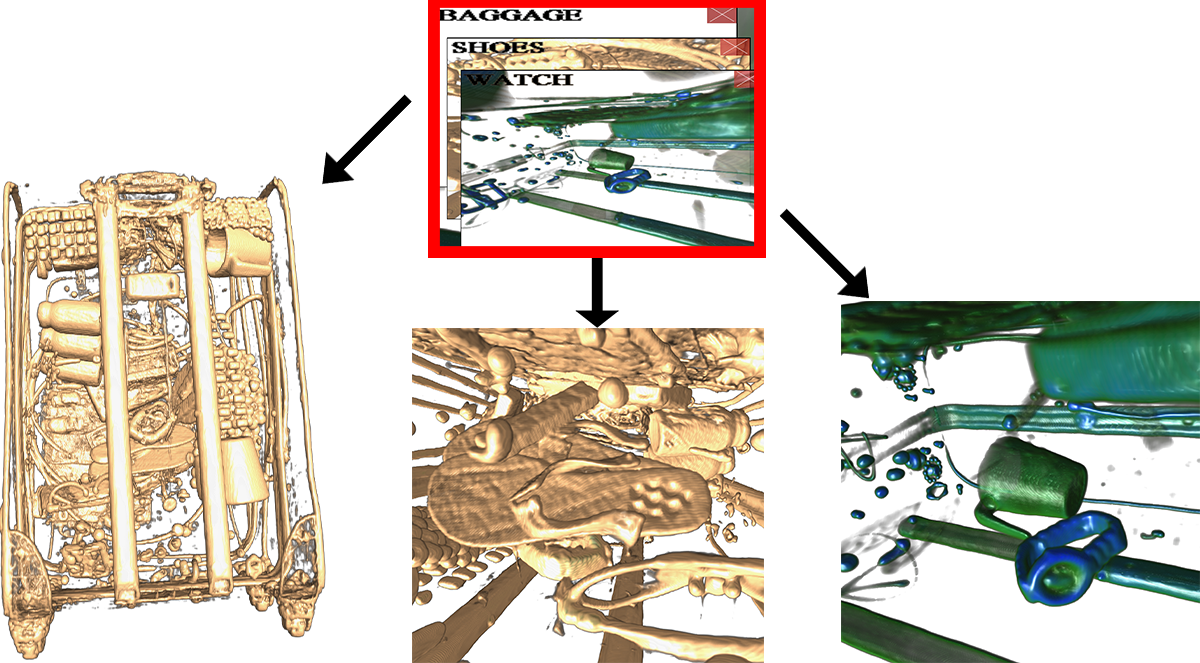
\includegraphics[width=9cm]{Figures/snapshots.png}
	\caption{ The labelled snapshots taken by the user representing objects of interest}
	\label{f:snapshots}
\end{figure}

\subsubsection{Dual temporal instance navigation}

Our system provides many animated transitions when the user explores the baggage (change of point of view, transfer function modification, item selection...) like \cite{tversky_animation:_2002}. To ease user's navigation, we added two temporal instances representing the states before and after an automatic modification of the visual configuration. This interaction is based on the undo-redo paradigm. On the top right of the main window, we added two views representing the previous state before the transition and the final one after the transition. One can navigate through this transition by dragging from one state toward the other one. The more the cursor gets close to the center of a state, the more the current view gets close to its configuration. The user can also click on the desired state to directly assign its visual configuration (\autoref{f:temporal}).
 \begin{figure}
 \centering
	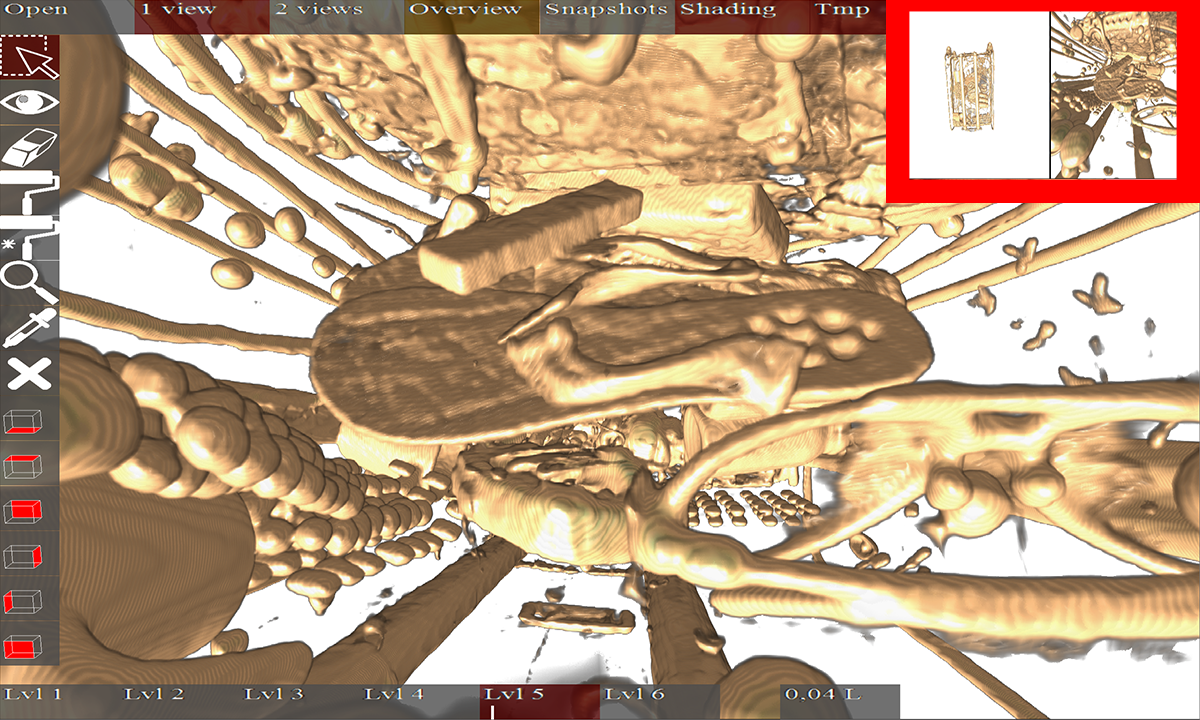
\includegraphics[width=9cm]{Figures/temporal.png}
	\caption{ The labelled snapshots taken by the user representing objects of interest}
	\label{f:temporal}
\end{figure}

\subsection{Possible Use Cases}

This section presents two scenarios that underline our system assets. The first scenario illustrates how users can explore a suspicious baggage and address occlusion to inspect items inside. The second scenario shows how to visualize the content of a closed metallic container. Currently, most airport don't use 3d systems, so we propose possible scenarios to highlight  how the usefulness of our interaction techniques.

\subsubsection{	Inspection of a suspicious baggage }
When a baggage arrives, the user sees it in its initial appearance which mainly shows the global structure . In order to better perceive its content, the user explores  the different transfer function presets. He or She clicks on the first level, then drags the cursors toward the others. This manipulation aims to reveal high density items hidden by those with low density 

(\autoref{f:scenario1_1}).
\begin{figure}
\centering
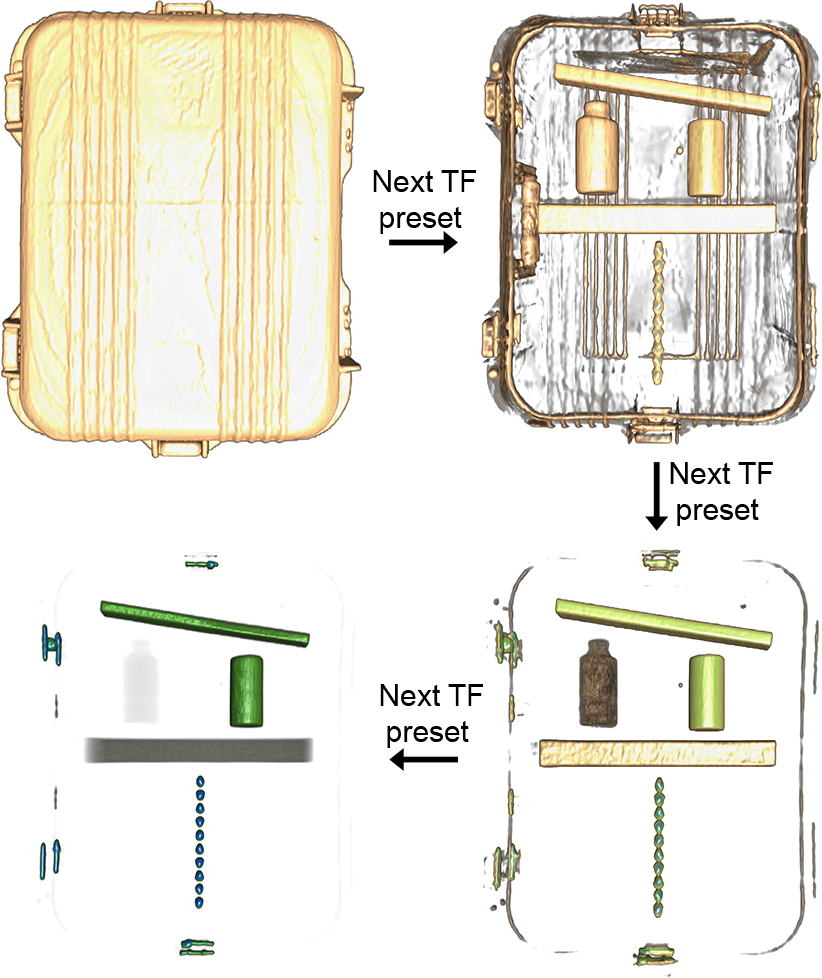
\includegraphics[width=9cm]{Figures/scenario1_1.png}
\caption{ The transfer function presets help the user perceive the different types of material inside the baggage }
\label{f:scenario1_1}
\end{figure}    
Once the user has a global understanding of the baggage, it seems to be a parcel bomb. So he or she decides to further inspect some specific areas. For instance, the user focuses an object which looks like an explosive material. To estimate the potential damages that could be caused by this potential threat, the security agent lock the camera on it. This object is now the main object of interest, and all  manipulations (e.g. translation, rotation) are now done around this object. This object of interest stays visible even if other items are in front of it (\autoref{f:menace}). 

\begin{figure}
\centering   
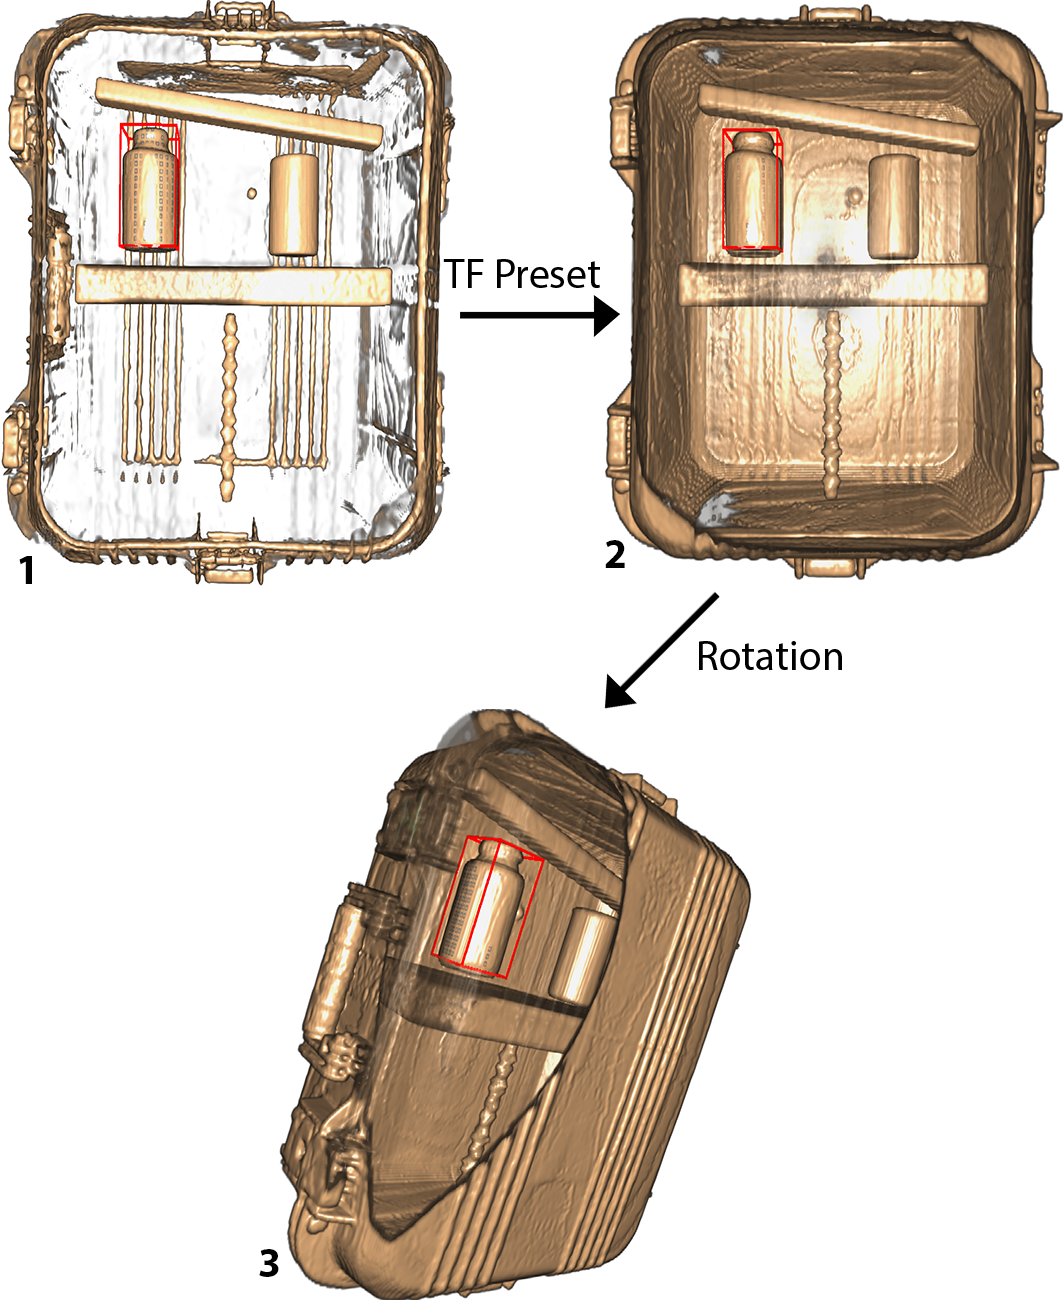
\includegraphics[width=9cm]{Figures/menace.png}
\caption[Inspection of an object from different perspectives.]{ Inspection of an object from different perspectives. 1- The user defines an object of interest for further inspection. This object is then inside a box with red borders. 2-  The user modifies the transfer function to see the target in another context. 3- The user rotates the baggage to look at the menace from a different perspective. It stays visible whatever the manipulation carried out.  }
\label{f:menace}
\end{figure} 


After the user finished this contextual inspection, he or she decides to inspect this object alone. To do so, the user selects it, and enables the second view. More information such as density and volume are displayed (\autoref{f:scenario1_3}).
\begin{figure}
\centering
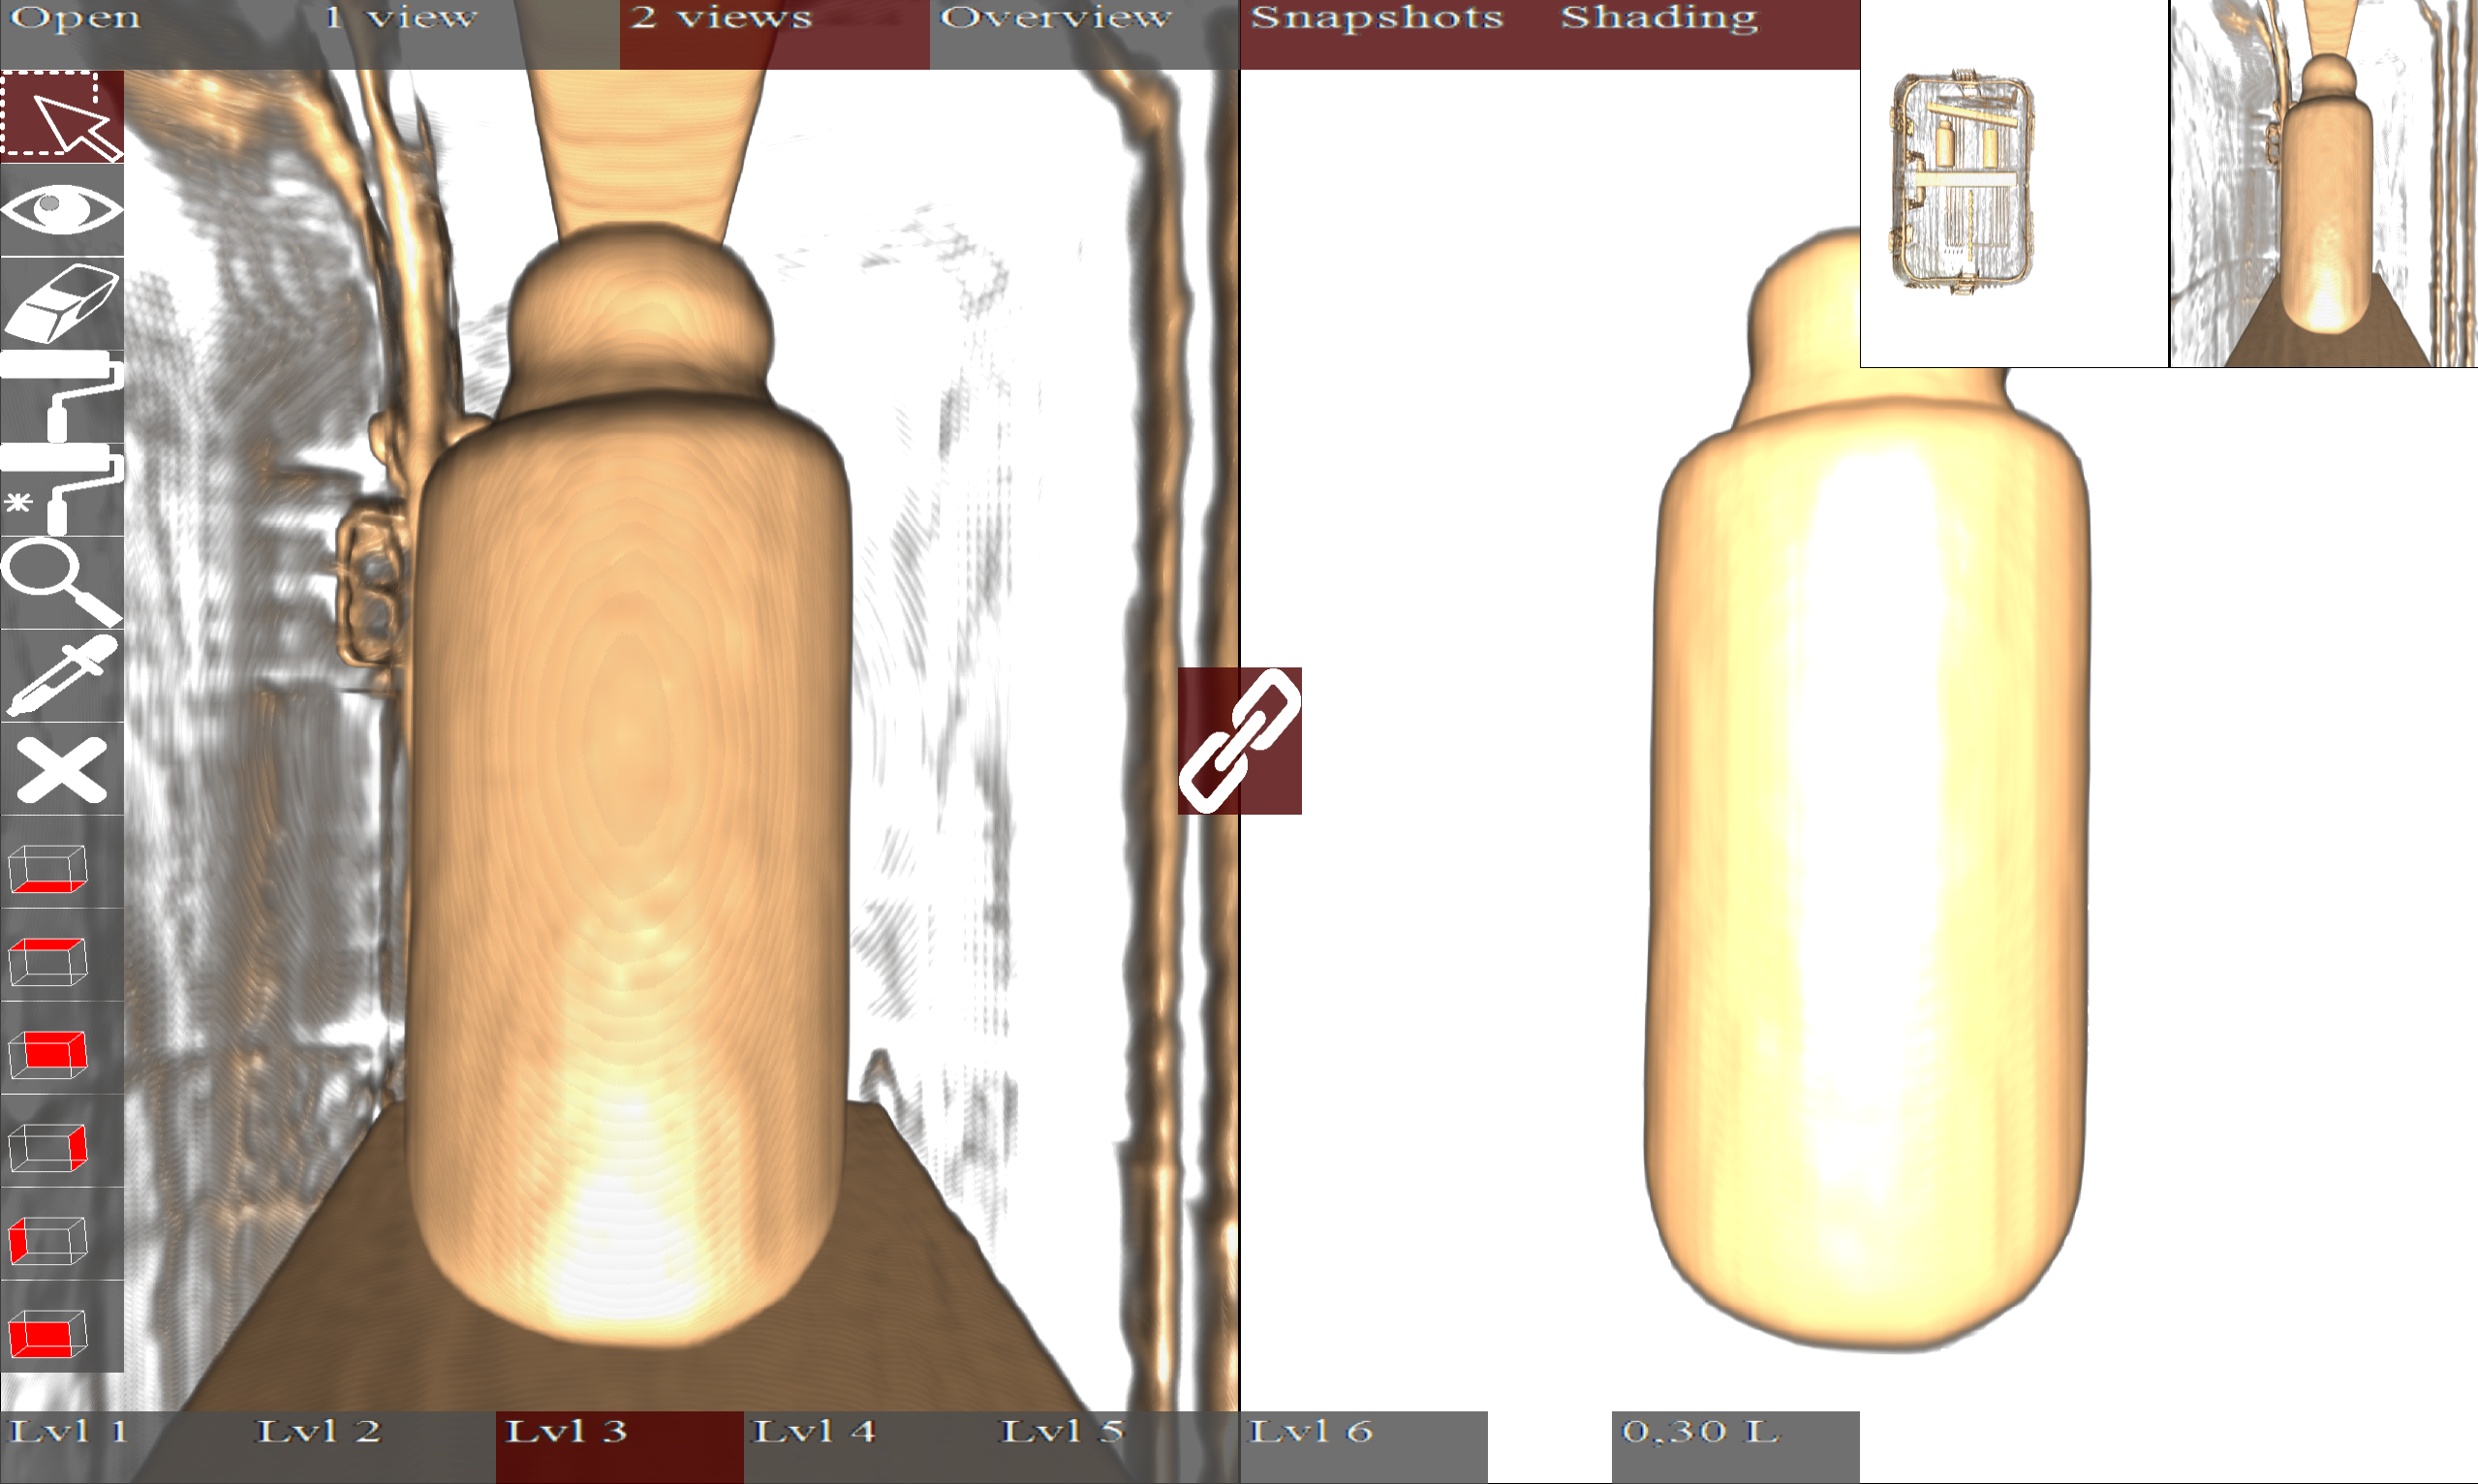
\includegraphics[width=7cm]{Figures/scenario1_3.PNG}
\caption{ A suspicious object is inspected apart of the rest of the baggage }
\label{f:scenario1_3}
\end{figure}

\subsubsection{Inspection of a big metallic object}

In this scenario, the user inspects a baggage featuring many visual artifacts which could be considered as noise (\autoref{f:scenario2_1b}). These spikes are created by the reflection of the x-rays on the heavy materials. Therefore, these visual artefacts are a hint indicating the presence of large metallic object. The user navigates through the different transfer function presets (\autoref{f:scenario2_2}) .
 
\begin{figure}
\centering
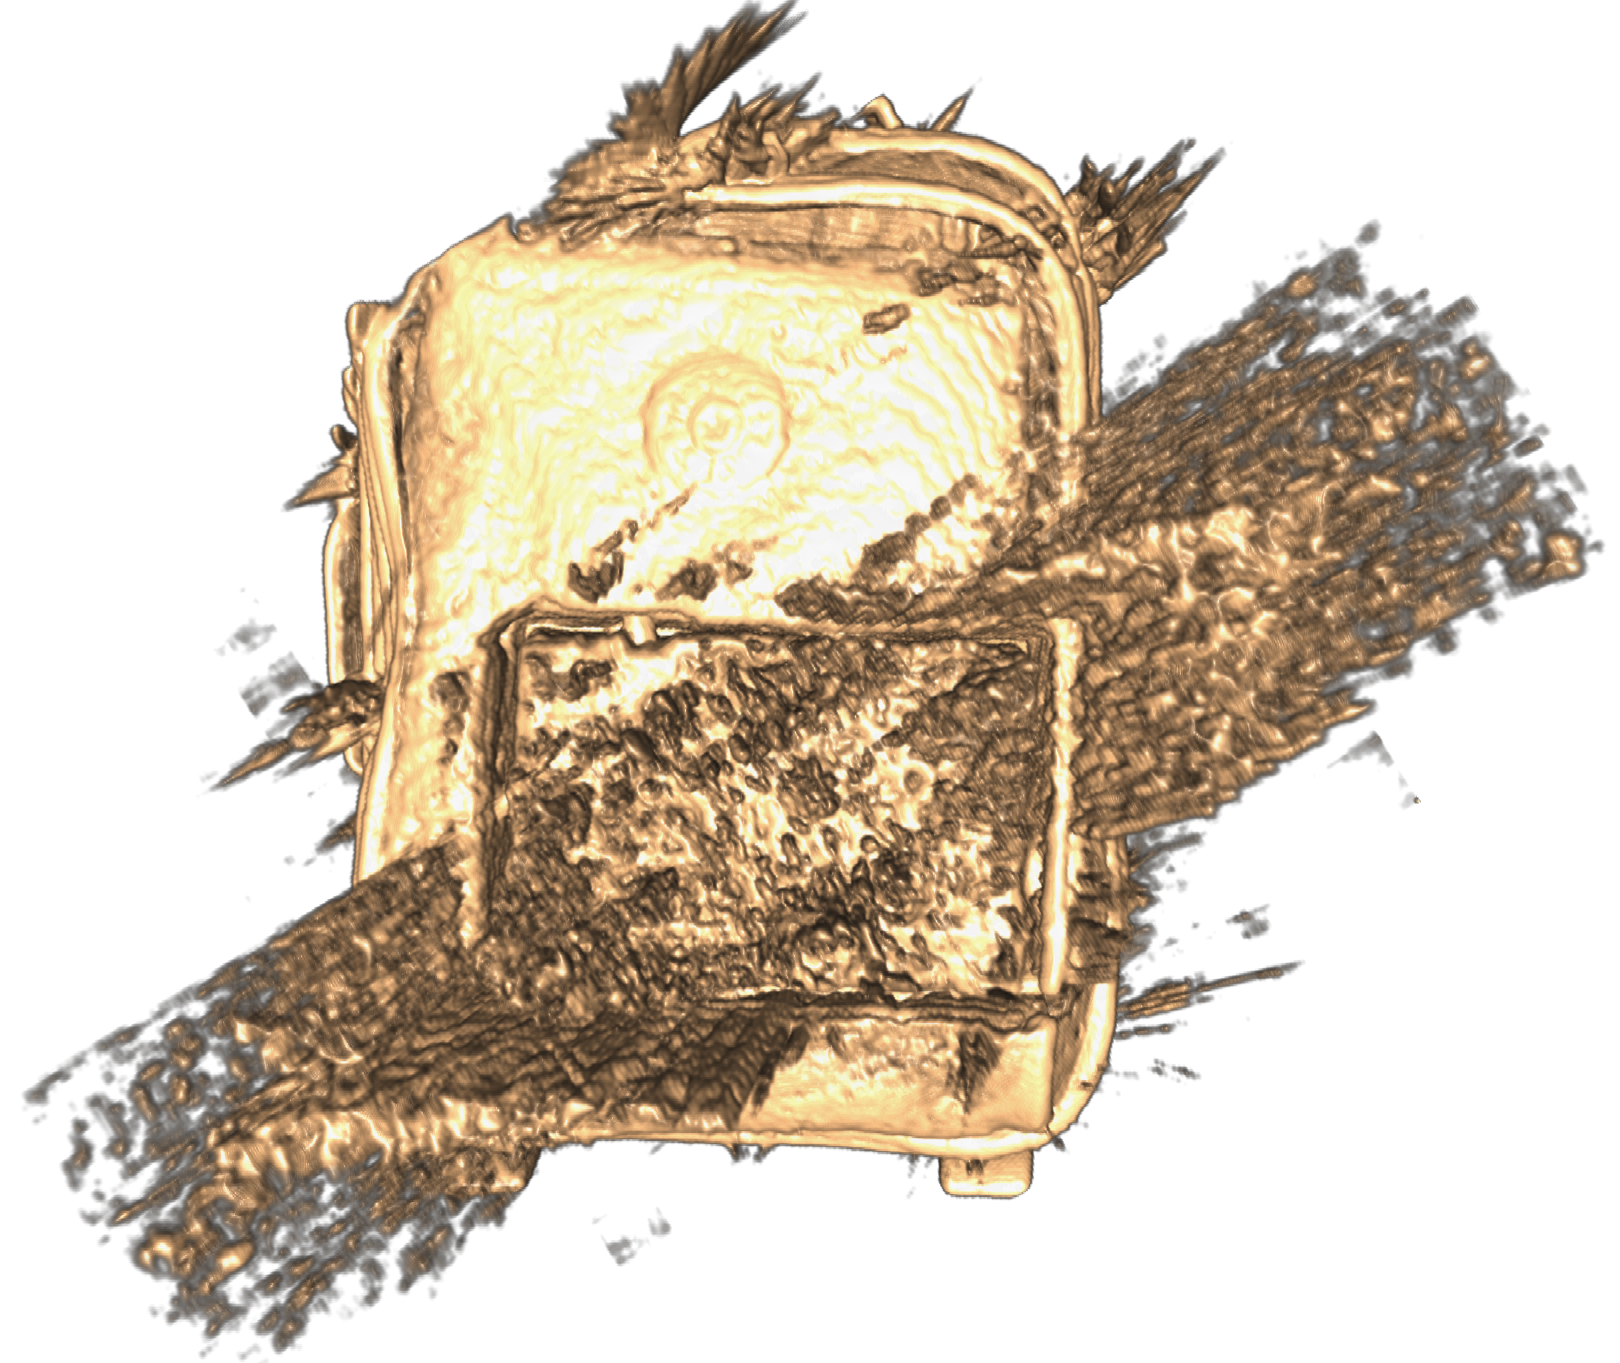
\includegraphics[width=9cm]{Figures/scenario2_1.PNG}
\caption{ Noise due to the presence of a big metallic object }
\label{f:scenario2_1b}
\end{figure}
After the selection of the adequate transfer function setting, he or she decides to farther inspect this metallic object. To do so, the user selects it with a double clicking on it. This object seems to be an engine.
\begin{figure}
\centering
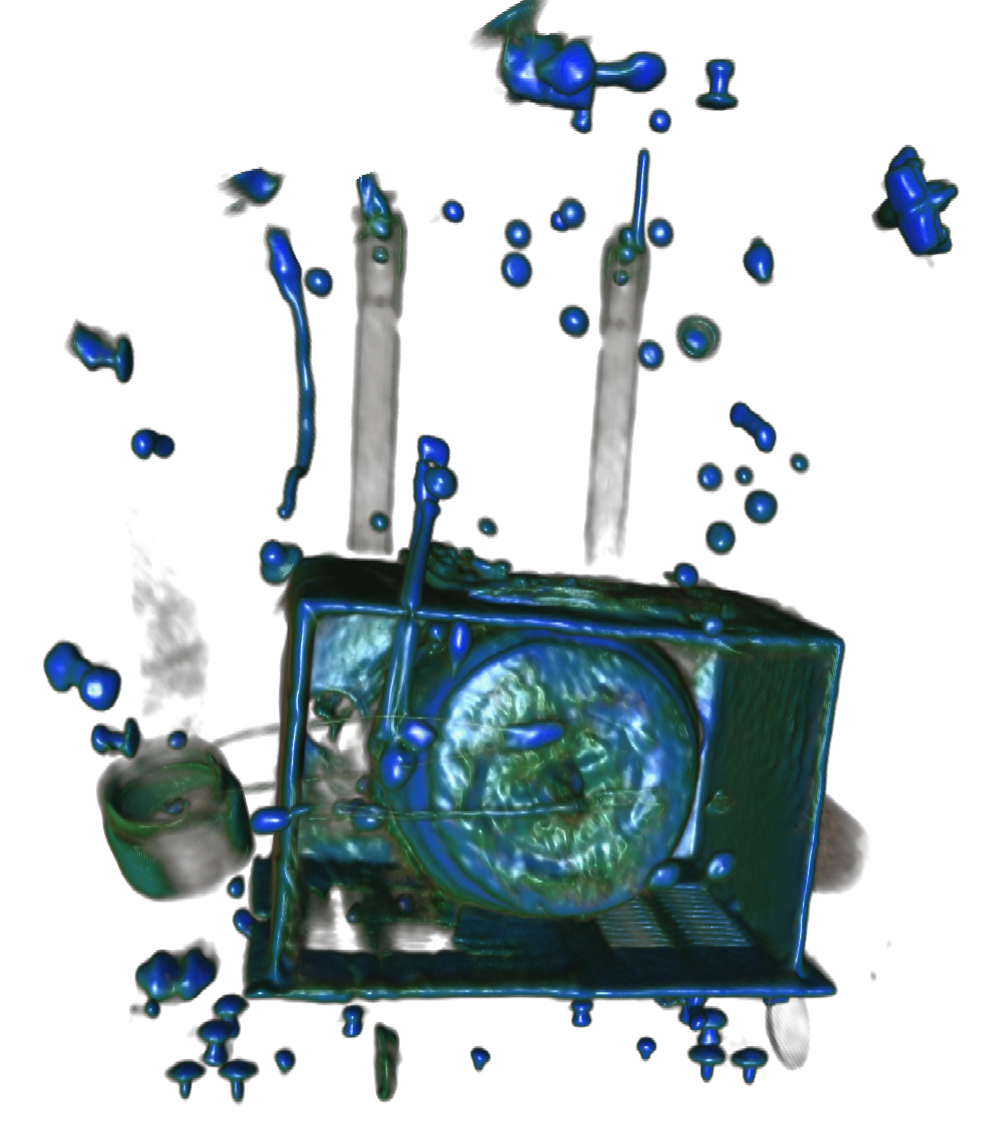
\includegraphics[width=9cm]{Figures/scenario2_2.PNG}
\caption{ The baggage actually contains  an engine }
\label{f:scenario2_2}
\end{figure}

In order to find out whether this engine is empty or not, the user decides to brush its half and to see its content. The user activates the brush tool, and while holding down the right button of the mouse, he or she brushes to remove the undesired section. After the brushing is carried out, the user modify the transfer function to show the lowest densities(\autoref{f:scenario2_1}).
\begin{figure}
\centering
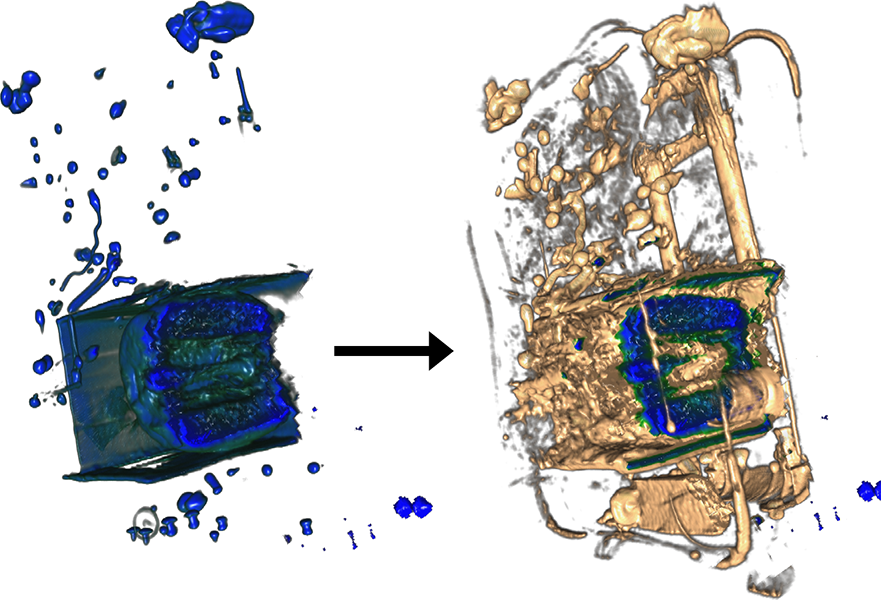
\includegraphics[width=\textwidth]{Figures/scenario2_3.png}
\caption{ the user reveals some low density materials inside the engine }
\label{f:scenario2_1}
\end{figure}


\subsection{Technical Constraints and Implementation}

Tomographs generate files which contain all the densities encountered by the x-rays through the baggage. These files usually contains around 30 million values. To load and to display such dataset in an interactive system, we used the parallel computation power of the graphic card. We used a program written in C\# combined with the CUDA parallel computing platform and a set of GPGPU techniques. To display the dataset, we used a standard ray casting algorithm. The contributions of you work rely on new interactions and their associated algorithms. This section will detail their implementations.

\subsubsection{Object selection}

Our software features interactive selection and voxel manipulation functionalities. To implement these interactions, we had to find a way to extract objects from the volume data. To do so, we explored many object detection algorithms such as contour trees by \cite{carr_computing_2000} and branch trees by \cite{pascucci_multi-resolution_2004} algorithms. But, according to the literature and our experience, these algorithms are computationally expensive and time-consuming especially during the preprocessing steps. In addition, this algorithm needs many settings and modifications to process the variety of available possible items which compose a baggage. For these reasons, we developed our own selection algorithm, see \cite{hurter2017object}. It is based on a simple brute force multi-threads propagation algorithm. The first step consists in casting a single ray toward the volume data where the selection need to start.
Consider the typical DVR algorithm: Given a scalar volume $V \subset \mathbf{R}^3 \rightarrow \mathbf{R}$, each pixel $\mathbf{x} \in I$ in the DVR image $I \subset \mathbf{R}^2$ thereof corresponds to the compositing of sampled data along a ray that passes through $V$ and ends at $\mathbf{x}$. Such rays are defined by the eye position $\mathbf{e}$ and a ray direction unit vector
\begin{equation}
\mathbf{d} = \frac{ (\mathbf{x} - \mathbf{e}) }{ \| \mathbf{x} - \mathbf{e} \| }
\end{equation}
as the equation of a ray passing through a pixel is :
\begin{equation}
\mathbf{x}(t) =  \mathbf{e} + t\mathbf{d}
\end{equation}
where $x$ is the float-point location of the window corresponding to the pixel.
 We stop its progression as soon as it hits a visible voxel.



Second, we propagate the selection in every directions. For each encountered voxel, we check whether it is visible according to the current transfer function . If the voxel is visible we go on with the selection propagation. We spread within the baggage by launching many threads starting from the location where the first visible voxel has been hit. The number of thread depends on the number of logical processors inside the current hardware. Each thread checks whether its neighbors are visible, and keep spreading towards the visible voxels. This propagation algorithm stops whenever there are not any more visible voxels to spread into ( algorithm \autoref{alg:propagation}).

\begin{algorithm} \caption{Pseudo code for the selection propagation} 
\label{alg:propagation}
\begin{algorithmic}[1]
\Require $V$ the volume

\State Cast a ray toward the volume $V$  
\State  pt $\leftarrow$ intersection point between the ray and the volume \;
\State  finished $\leftarrow$ false \;
 \If{pt exists}
 	\State step $\leftarrow$ direction toward the volume \;
    \While{pt is inside the volume and $!$ finished }
  	\State color $\leftarrow$ the color at pt \;
  \If{color.alpha $>$ 0 }
	\State \emph{// spread into neighbors}
    
    \State v $\leftarrow$ current voxel \;
	\While{ v has neighbors }
    	\State color $\leftarrow$ voxel's color \;
        \State grad $\leftarrow$ voxel's gradient\;
    	 \If{color.alpha $>$ 0 and grad $<=$ threshold }
         \State 	v.selected $\leftarrow$ true \;
         \EndIf
        \State  v $\leftarrow$ next neighbor \;
    \EndWhile    

    \State finished $\leftarrow$ false;
    
  \EndIf
 \State  pt $\leftarrow$ pt + step \;
\EndWhile
 
\EndIf

\end{algorithmic}
\end{algorithm}




\subsubsection{Occlusion minimization}

Once the item of interest is selected, our system animates the visual configuration to display a new point of view of the selection which minimizes object occlusions. To do so, the system first computes the selection bounding box composed of six faces. Then, the system computes the six possible point of views. For each of them, the system counts the number of visible pixels which display the selected object. This is done thanks to the ray casting algorithm which propagates though the data cube and thus can test if the ray hits the selected items without any occlusion. Finally, the system defines the appropriate point of view as the bounding box face with the highest number of visible pixels of the selected item, see \cite{hurter2017selective}.
The system can then animate the volume visualization toward this new visual configuration and update the two temporal instances (before and after the pan, zoom and rotation modifications).

\subsubsection{Extended brushing technique}

The extended brushing techniques help the user explore the volume without modifying the transfer function. This interaction is also based on the ray casting algorithm. We only cast the rays located inside the radius of the brush in a parallel way.
When a ray hits a visible voxel whose density is within the brushing range, this voxel is then removed. If the voxel density is not in the brushing range, the ray casting algorithm stops.
The cancellation of the brushing is quite similar to the previous algorithm. The rays start from the back of the volume toward the front instead of front-to-back. The second difference consists in restoring the voxels whose density is inside the range.

\subsection{Discussion and conclusion}

Since we developed this system with four baggage security practitioners, we had the opportunity to validate the usefulness of each developed technique. Through an interactive process, the users gave their feedbacks all along the development process which helped to assess and to guide the proposed interaction techniques. Feedback was mainly positive and the user did not face any specific difficulty to use our system. Users mainly appreciated the simple interface with few widgets and the reduced set of interactions. Surprisingly, users were very interested to use the transfer function. The histogram and its transfer function were also appreciated even if the corresponding technique is not simple to understand. We suppose that our interface motivates users to learn more regarding the technique behind it. Users also mentioned the need to display the actual density (the numerical value) of selected object. They also ask many times if the displayed color corresponds to the one currently in use in operational settings. This confirms the fact that users are willing to keep some existing features and prefer to use a system they are already familiar with.
The users also appreciated our design requirements with smooth transitions and incremental investigations of baggage.
\par All of these observations and qualitative evaluations deserve to be validated through proper evaluations which are out of the scope of this user study.
Our system is fully functional and interactive enough to perform baggage explorations. Many improvements can still be done in order to improve its usages in terms of new interactions and exploration time reductions.
Technically speaking, the selection of the adequate point of view can be improved with more than 6 investigated faces. But in practice, this simple paradigm remains suitable. If the computed point of view is not fully satisfactory, one can manual rotate the baggage. Nevertheless, the developed algorithm will not necessary provide the best solution (the lowest occlusion) but a satisfactory one.
\par Our goal was to develop
innovative interactions to support baggage exploration but we did not really took into account the optimization of the exploration duration time. Manipulating the 3D volume may take time as well as our new interaction techniques. We think that these techniques have a great potential but they are suitable to explore in more details a suspicious baggage. Existing investigation techniques (with the 2D flattened image) are suitable to quickly and efficiently detect ''clean'' baggage. Then our tools can be a good solution to further investigate a potential threat with more available time.